\documentclass[letterpaper,12pt,fullpage]{article}

\usepackage[left=1in,right=1in,top=1in,bottom=1in]{geometry}
\usepackage{cite}
\usepackage{graphicx}
% \usepackage[dvips]{graphicx}
% \usepackage{epsfig} % for postscript graphics files
  % \graphicspath{{../eps/}}
% \DeclareGraphicsExtensions{.eps}
\usepackage{amsmath}
\usepackage{amssymb}
%\usepackage[cmex10]{amsmath}
%\usepackage{array}
%\usepackage{mdwmath}
%\usepackage{mdwtab}
%\usepackage{eqparbox}
\usepackage[tight,footnotesize]{subfigure}
%\usepackage[caption=false]{caption}
%\usepackage[font=footnotesize]{subfig}
%\usepackage{fixltx2e}
%\usepackage{stfloats}
\usepackage{hyperref}

% correct bad hyphenation here
%\hyphenation{op-tical net-works semi-conduc-tor}

\input latex-commands

\newcommand{\gc}{{\mbox {GravityCompensation}}}
\newcommand{\invdyn}{{\mbox {\tiny ID}}}

\newcommand{\shrinkfig}{\def\baselinestretch{1.0}\small} % 0.9 okay
\newcommand{\shrink}{\def\baselinestretch{1.1}\small} % 0.97 % 0.95 okay

\begin{document}

\title{A Survey of Possible Exoskeleton Control Architectures and
Algorithms\\
(Draft 2.2)}

\author{Alex Ansari, Christopher G. Atkeson, Howie Choset, and Matthew Travers\\
Carnegie Mellon University}

\maketitle

\begin{abstract}
Abstract to be written.
\end{abstract}

\section{Executive Summary}

Executive Summary to be written.

\section{Scope: What is this paper about?}

This paper surveys possible exoskeleton control architectures and
algorithms.
One goal is to address the question:
{\it How do exoskeleton control approaches compare with 
approaches to humanoid robot control?}
A companion paper surveys implemented exoskeleton control architectures
and algorithms~\cite{}.

The focus is on exoskeleton control that allows a
highly trained and top percentile athletic 
operator to carry a payload that weighs approximately the same amount
as the operator. We envisage these types of exoskeletons to be useful
in carrying protective and safety equipment for SWAT teams, police,
firefighters, and soldiers. 

We expect each exoskeleton controller
to be used by and optimized for a single operator.
A substantial investment in capturing the operators normal behavior,
operator training and learning, and controller customization can be made.

We focus this survey on exoskeleton control for lower body tasks (standing, walking,
running, jumping, kicking, dodging, ...).
We do not survey exoskeleton control for human arms or manipulation. 

We treat the torso and helmet of the exoskeleton as the payload,
and focus on a lower body exoskeleton to support any payloads that
are on the torso or head.

%\section{Symbiosis and Autonomy, Handling Errors, and Superhuman Reflexes}
A later white paper will discuss
possible combinations of response to user and exoskeleton
autonomy including balance control; response to trips, slips,
stumbles, and fumbles; task assistance and guidance (guide operator to
doorknob, button, or light switch); superhuman response to external
perturbations such as projectiles and explosions; and autonomous
execution (operator/exoskeleton symbiosis with multi-tasking)?

A later white paper will discuss how to handle malfunctions and damage to the
system. Basically this boils down to fault detection, and switchover to
an approapriate safe mode of operation.

\subsection{Let's keep it simple}

Terms like impedance and admittance control are used, but are often confusing,
as in controller design one can choose from several possible
inputs into the exoskeleton (exoskeleton positions,
velocities, accelerations, operator-exoskeleton contact forces and
exoskeleton-world contact forces), and choose from several possible exoskeleton
outputs: exoskeleton actuator forces and torques, exoskeleton
motion (position, velocity, and acceleration), as well as operator-exo
contact forces or exo-world contact forces.

A useful background paper on impedance and admittance:\\
\url{http://summerschool.stiff-project.org/fileadmin/pdf/1804_C19.pdf}

Variants of nonlinear feedback control such as feedback linearization or
sliding mode control are largely ignored in this paper.
Once the decision to use feedback control
based on a set of observable quantities and with particular outputs is made,
one can try out the various linear and nonlinear feedback control paradigms
to see what works well.

Variants of function approximation methods such as lookup tables, fuzzy logic,
sigmoidal neural networks, radial basis functions, and locally weighted regression
are also largely ignored. Once the decision to use a function approximator
and what the inputs and outputs are has been made, one can try out the various
approaches to see what works well.

Same for optimization methods.

Same for constraint enforcement (such as avoiding self-collisions)
in either optimization or feedback control (barrier
Lyapunov functions (BLF)~\cite{IEEE06911561}).

Stability proofs of any of these methods should be viewed skeptically due
to the unmodeled operator-exoskeleton and exoskeleton-world contact dynamics, 
actuator unmodeled dynamics, joint play and exoskeleton
structural deformation, and controller
time delays which are typically ignored, especially in proofs involving
passivity arguments or Lyapunov functions.
We ignore stability proofs as well.

\section{What are some design philosophy alternatives?}

\subsection{``Invisible'' exoskeleton}

Can we build an exoskeleton allows the operator to behave naturally
and exerts little or no force on the operator?

This could be achieved through active control using feedback of the
operator-exoskeleton forces. Additional gravity, friction, actuator, and
inertial compensation (inverse dynamics) can improve performance.

\subsection{``Natural'' exoskeleton}

Can we build an exoskeleton allows the operator to behave naturally?
The operator can feel the exoskeleton, but can overpower it when necessary.

Bypass valves and clutches could allow the operator to physically ``take over''
and push the relatively lightweight leg mounted exoskeleton around.

``Passive'' degrees of freedom can have physical or ``virtual'' springs
applied to assist in support (all abduct/adduct DOF, rotational DOF).
These aids can be clutched out or turned off when necessary.
``Virtual'' springs (springs implemented actively through exoskeleton
actuators) can be modulated.

\subsection{``Symbiotic'' exoskeleton}

Can we build an exoskeleton that allows the operator/exoskeleton team
to be effective, but not necessarily behave naturally? 
The operator needs to learn to ``fly'' the suit,
just as operators learn to operate parachutes,
wing suits, diving equipment, high and low temperature protective
suits, firefighting equipment, and high altitude flight
and parachute suits.

The exoskeleton can adapt its behavior to the task.
For example, for jumping, the exoskeleton can operate like a pogo 
stick:\\
\url{https://www.youtube.com/watch?v=lbp41vWP4o4},\\ 
and for running it could act like jumping stilts:\\
\url{https://www.youtube.com/watch?v=9ZOd7yEyhwI},

\section{Effects of underlying exoskeleton actuator technology}

One basic distinction is whether the actuators are thought of as position
or force sources. Often this is revealed by the design of the ``low level''
controller. Note that this is often somewhat confusing. Electric motors
are torque sources (low impedance), but when a high gear ratio transmission
is added (such as a harmonic drive) the whole system becomes high impedance
and thus is best thought of as a position (or velocity) source. Therefore,
position or velocity 
control is performed by the low level controller. Hydraulic actuators
are high impedance, but when a force or load sensor is added (or piston differential
oil pressure is used as a force sensor), the whole system becomes low impedance
and is best thought of as a force source. Force (or joint torque) control is
performed by the low level controller. Force or torque sensing can be added to an
electromechanical drive train (electric motor plus gears or electric
motor plus ballscrew)
to make it lower impedance and more like a force source as well.

\section{Recommended Control Architecture}
\label{sec:architecture}

We recommend the following hierarchical control architecture~\cite{IEEE06907051}:

{\bf Low Level Control:} Present interface to actuators and
high bandwidth feedback control, degrees of freedom,
or synergies of either:
\begin{itemize}
\item
Position control.
\item
Pure force or torque control.
\item
Impedance control: specify desired position (for spring), and generate
stiffness, damping, and potentially a modified inertia or moment of inertia.
Modifying inertia is more dangerous than providing active stiffness
or damping.
Or (almost equivalently),
specify a desired force and change the force according to position, velocity,
and acceleration.
\item
Online optimization of accelerations, actuator forces and torques, and contact forces
using quadratic programming.
\end{itemize} 
One important synergy is coordinated control of the center of mass location and
velocity for balance.
PID or fancier feedback control laws are implemented at this level.
Gravity, friction, actuator dynamics, and other feedforward disturbance
compensation are implemented at this level, as well as any inverse dynamics
or other types of feedforward reference tracking control.
Disturbance observers for model errors and contact/wind forces
are implemented at this level.
Typically this is done by a high sampling rate global servo~\cite{Atlas-robot}
or distributed limb or joint-level high sampling rate servos~\cite{Sarcos-robot}.
Often, this controller is provided by the manufacturer of the robot
or exoskeleton and runs on a separate computer system from the
``user's'' or task/application controller~\cite{Sarcos,Atlas}.

{\bf ``Phoneme'' Control:} Mid-level controllers
for relatively constant phases of behavior.
Often involves position or velocity targets (goto or
stay-at X), trajectory references, ...
Example from walking: left-stance, double-support-1, right-stance, double-support-2, ...;
Example from running: left-foot-down, flight-1, right-foot-down, flight-2, ...;
Example from horizontal jumping: hjump-pushoff, hjump-flight, hjump-prepare-landing, hjump-impact, hjump-balance, ...;
Finer resolution may be needed. For example a walking stance period may
be broken up into heel-strike, first-half, second-half, pushoff, and toe-off.
The first and second halves of stance are divided by when the center of mass
passes over the ankle.
Local inverse kinematics (finding small joint motions for small target changes)
is performed at this level.
This level often provides the behavioral primitives or ``verbs'' for robot programming.

{\bf ``Word'' Control:} Mid-level controllers for sequences of ``phoneme'' behavioral
units.
Often involves finite state machines, timers, if-then condition testing, gain
scheduling, ...
Examples: walk-to-location(x=7.8m, y=2.3m), run-to-location(speed=3.7m/s),
horizontal-jump(height= 2m, length= 5m).
Global inverse kinematics (selection of solution branch) is performed at this level.
This level often determines the control flow of a behavior.

{\bf Highest Level Control} aka {\bf Behavior Selection:} 
Answer the question: ``What do I do next?''
Select behaviors and behavioral parameters (targets,
speeds, durations).
Often involves finite state machines. timers, if-then condition testing, ...
This level often involves a great deal of human operator online interaction,
or is completely done by the operator.

{\bf Error Handling:} Errors must be detected and handled by parameter (target)
adjustment and/or behavior switching
at all of these levels.

{\bf State Estimation:}
In this architecture, state estimation to deal with sensor noise and incomplete or
redundant sensing is a separate process and is as independent as possible
from the control method~\cite{certainty-eq,separation-prin}.
This makes evaluating different control methods much easier.

The recommended control architecture is intuitive, abstracts the hardware 
and lower level control in a straightforward way, is easy to program, and is
commonly used. Variants of this architecture were used by almost all teams
in the DARPA Robotics Challenge~\cite{}.

Closely related control architectures combine Phoneme and Word control,
or combine Phoneme, Word, and Behavior Selection.
This is not a major design change.

An alternative behavioral architecture might not have explicit levels but instead
has a ``soup'' of behaviors that compete or cooperate for the ability to
control the robot or exoskeleton. Subsumption architecture and other behavior-based
architectures are closer to the ``soup'' approach and to some extent
use inhibition and excitation
among behaviors to select active behaviors.

Another alternative behavioral architecture does not have explicit separate behaviors,
but one or a small number of functions or policies. 
We are seeing more of these architectures
due to the success and popularity of function approximation such as
deep learning.

An alternative approach to state estimation is to design state estimation
and control laws simultaneously~\cite{LQG-LTR}. Another alternative is
to have a controller with internal state, and design or learn a policy
that works well, but does not have an explicit state estimation 
part~\cite{lead-lag}.

\section{Exoskeleton dynamics}

Exoskeletons are similar to robots, but there are several important differences.
There are two sets of contact forces: operator-exoskeleton (which we denote
with a subscript $o$ as in $\vf_o$) and exoskeleton-world (which we denote
with a subscript $w$ as in $\vf_w$). If the operator is tightly strapped or
rigidly held by other types of physical constraints, we can lump the operator
body parts with the exoskelton parts which they are attached to in terms
of link inertias, locations of center of mass, and moments of inertia,
and just think of the whole system as one robot.
We can also separate out the operator dynamics if this is more convenient
(we separate them out and ignore them in what follows).
If the operator is loosely connected to the exoskeleton, this introduces a
huge modeling and control problem, and would also be very dangerous for the
operator (as riding a bull or bucking horse in a rodeo is dangerous to a rider).

The dynamics of a revolute exoskeleton are:
\begin{equation}
\mM(\vq) \ddot{\vq} + \mC(\vq,\dot{\vq}) + \mG(\vq) + \mF(\vq,\dot{\vq})
+ \mJ_w^{\tr}(\vq) \vf_w = \vtau + \mJ_o^{\tr}(\vq) \vf_o
\label{eq:dynamics}
\end{equation}
where $\vq$ are the joint angles and position of the ``root'' of
the exoskeleton, $\dot{\vq}$ and $\ddot{\vq}$ are the corresponding
velocities and accelerations, $\mM$ is the inertia matrix, $\mC()$ are the Coriolis and
centripetal forces, $\mG()$ are the gravitational forces, $\mF()$ are the
friction forces, $\mJ_w^{\tr}(\vq) \vf_w$ (Jacobian matrix multiplied with the
contact forces)
are the exoskeleton-world
contact forces 
expressed as exoskeleton joint torques, 
$\vtau$ are the exoskeleton
joint torques,
and $\mJ_o^{\tr}(\vq) \vf_o$
are the operator-exoskelton forces expressed
as exoskeleton joint torques.
$\vtau$ is augmented with zeros corresponding to the dimensions of $\dot{\vq}$
that correspond to root velocities, since those dimensions are not actuated.

To understand these equations better, it is useful to have all Jacobians equal
to the identity matrix. This means the operator is directly applying torques
at the exoskeleton joints ($\vtau_o$) (a realistic assumption), 
and so is the world ($\vtau_w$) (a very unrealistic assumption). In this case:
\begin{equation}
\mM(\vq) \ddot{\vq} + \mC(\vq,\dot{\vq}) + \mG(\vq) + \mF(\vq,\dot{\vq})
+ \vtau_w = \vtau + \vtau_o
\end{equation}

Note that we are ignoring the operator dynamics and operator muscle and tissue
forces resulting in operator joint torques. We will add these in later (or maybe
we won't ???).

We are also ignoring actuator dynamics, which we can handle by augmenting 
the state vector.

[SOMETHING ABOUT MODELING HUMAN + EXOSKELETON + WORLD ]

\section{Test case: Atlas humanoid robot}

Gazebo and SDFast models.

\section{Passive control with no active control}

One control option is to use only passive controls, and no active controls
or actuators.
Such a system would rely on counterbalancing, mechanical springs, air springs, etc.
to reduce forces. 
An operator would rely on mechanical backdrivability to drive
exokeleton to do tasks.
In this case, 
$\vtau$ is generated by passive devices such as springs or dampers.

\section{Open loop control}

Another control option is open loop control, in which actuator commands are
constant, or a function of time or phase of a behavior or task
(at least on the small time scale).
Commands or behaviors may be selected at a relatively coarse time interval
by the operator or by the exoskeleton controller.
This approach typically 
uses position and velocity control in either joint or
Cartesian coordinates
with either pre-generated references, selected targets,
or online generated trajectories to move to targets or perform tasks.
The operator relies on mechanical backdrivability 
to correct exoskeleton behavior.
In this case, it is common to generate the exoskeleton actuator commands using
a time or phase index:
$\vtau = \vtau_{ff}(t)$ where $\vtau_{ff}$ is a time
dependent feedforward torque vector.

Recognizing/estimating phase goes here.
Phase Triggered References could go here.
\begin{verbatim}
H.Kawamoto and Y.Sankai, “Power Assist Method Based on Phase
Sequence Driven by Interaction between Human and Robot Suit,”
Proceedings of the IEEE International Workshop on Robot and Human
Interactive Communication, pp. 491–496, 2004.
\end{verbatim}

Motion capture, motion libraries goes here.

Often finite state machines whose states correspond to left stance, double support 1,
right stance, and double support 2 are used to select behaviors. Gait transitions
can be triggered by foot touchdown and liftoff events, or
displacement of the Center of Mass (CoM).

Central pattern generator

Iterative learning control to acquire $\vtau_{ff}(t)$ for desired trajectories.

\section{Active gravity compensation}

Active gravity compensation is similar 
to counterbalancing or physical gravity compensation, except it is done
with exoskeleton actuators to cancel the exoskeleton weight (but not inertia).
\begin{equation}
\vtau = \hat{\mG}(\hat{\vq})
\end{equation}
where $\vtau$ are the exoskeleton joint torques, 
$\hat{\mG}()$ are the gravitational forces calculated using an imperfect model, 
and $\hat{\vq}$ is the estimated configuration of the exoskeleton,
The operator relies on mechanical backdrivability to drive
the exokeleton to do tasks.

Sarcos Primus Humanoid videos of active gravity compensation applied
to a humanoid robot:\\
CMU: cancel gravity and friction: \url{https://www.youtube.com/watch?v=Ac5cowTwOPw}\\
ATR: cancel gravity only: \url{https://www.youtube.com/watch?v=KNxxLm4sPys}

A simple approximation for a lower body exoskeleton with a heavy payload at the
torso is:
\begin{equation}
\vtau \approx \hat{\mJ}^{\tr}(\hat{\vq}) (\hat{m} \hat{\vg})
\end{equation}
where $\hat{\mJ}$ is the estimated Jacobian matrix,
$\hat{m}$ is the estimated
weight of the exoskeleton (which could include the operator),
and $\hat{\vg}$ is the gravity vector (it is estimated due to possible orientation
errors in the controller's estimate of vertical).
All weight is assumed to be concentrated at the center of mass of the full system.

\section{Friction compensation}

Friction can also be compensated.
\begin{equation}
\vtau = \hat{\mF}(\hat{\vq},\hat{\dot{\vq}}) 
\end{equation}
are the estimated friction torques at the estimated exoskeleton configuration
and velocity.
Note that these may be load dependent, and may require additional state to
correctly handle stiction and hysteresis effects.

Sarcos Primus Humanoid video of friction compensation applied
to a humanoid robot:\\
CMU: cancel gravity and friction: \url{https://www.youtube.com/watch?v=Ac5cowTwOPw}\\

\section{Online inverse dynamics control}
\label{sec:invdyn}

The goal here is to map from desired motion (in this case desired
accelerations) to exoskeleton actuator commands (and desired operator
and world contact forces).
The exoskeleton actuator torques
attempt to match the torques caused by inertial, Coriolis, centripetal,
gravitational, frictional, and exoskeleton-world contact forces.
\begin{equation}
\vtau = \vtau_{\invdyn} 
= \hat{\mM}(\hat{\vq}) \ddot{\vq}_d
+ \hat{\mC}(\hat{\vq},\hat{\dot{\vq}})
+ \hat{\mG}(\hat{\vq})
+ \hat{\mF}(\hat{\vq},\hat{\dot{\vq}})
+ \hat{\mJ}_w^{\tr}(\hat{\vq}) \hat{\vf}_w
\end{equation}
If there are actuator dynamics or other dynamics, we can include those
dynamics as well.

These force/torque estimates rely on estimated dynamic models and their parameters.
If the models and estimated state (position and velocity) are perfect, we get
perfect cancellation of most of the dynamics:
\begin{equation}
\mM(\vq) (\ddot{\vq} - \ddot{\vq}_d) = \mJ_o^{\tr}(\vq) \vf_o
\end{equation}
If $\ddot{\vq}_d$ is set to zero, the operator directly drives the acceleration
of the exoskeleton with an effective inertia of $(\mM^{-1}(\vq) \mJ_o^{\tr}(\vq))^{-1}$
\begin{equation}
\ddot{\vq} = \mM^{-1}(\vq) \mJ_o^{\tr}(\vq) \vf_o
\label{eq:cancel}
\end{equation}
$\ddot{\vq}_d$ can be used to drive the exoskeleton along trajectories, and
the operator can directly modify the trajectory.

Simplifying equation~\ref{eq:cancel} by 
assuming the operator directly applies torques at the
exoskeleton joints we get:
\begin{equation}
\mM (\vq) \ddot{\vq} = \vtau_o
\end{equation}
The operator sees the true inertia of the exoskeleton, but no gravitational
loads and no other dynamics (Coriolis, centripetal, or frictional).

Note that we cannot change the apparent inertia of the exoskeleton without
some form of acceleration or force feedback.
With acceleration feedback we can make the exoskeleton have a different inertia.
Setting $\ddot{\vq}_d$ to zero and adding acceleration feedback:
\begin{equation}
\vtau = \vtau_{\invdyn} - (\mM_d(\hat{\vq}) - \hat{\mM}(\hat{\vq})) \hat{\ddot{\vq}}
\label{eq:change-inertia1}
\end{equation}
sets the apparent inertia to $\mM_d$ if the dynamic models are perfect, and
the state estimation produces not only perfect positions and velocities but
also perfect acceleration estimates. In the case 
where the operator directly applies torques at the
exoskeleton joints we get:
\begin{equation}
\mM_d (\vq) \ddot{\vq} = \vtau_o
\end{equation}
In robotics this is usually considered a bad idea if $\mM_d$ is smaller (a complex
issue for a matrix) than $\mM$ at any $\vq$. This type of control is vulnerable
to unmodeled dynamics. However, in an exoskeleton, since we have not tried to
cancel the human's dynamics, the human stabilizes a possible unstable exoskeleton
(if the straps are tight enough).

With force feedback we can also make the exoskeleton have a different inertia.
Setting $\ddot{\vq}_d$ to zero and adding force feedback:
\begin{equation}
\vtau = \vtau_{\invdyn} + \mK \hat{\vf}_o
\end{equation}
In the case where the force measurements are perfect and 
the operator directly applies torques at the
exoskeleton joints we get:
\begin{equation}
(\mK + \mI)^{-1} \mM (\vq) \ddot{\vq} = \vtau_o
\end{equation}
By setting $\mK = \mM^{-1}_d (\vq) \mM (\vq) - \mI$ we can achieve
\begin{equation}
\mM_d (\vq) \ddot{\vq} = \vtau_o
\end{equation}

Online inverse dynamics control is a generalization of 
active gravity compensation to include
inertial, Coriolis, and centripetal forces (forces due to acceleration and
velocity), and potentially frictional forces.
Online inverse dynamics can be added to open loop behavior execution
and many other types of control such as operator force
feedback control, impedance control, and admittance control.
Computed torque control and feedback linearization are forms of online
inverse dynamics.

A key question is where does desired acceleration come from?
\begin{verbatim}
  Operator force control.
  Receding Horizon Control of optimal trajectory of 
    idealized LIPM+flywheel model (Atkeson)
  intent prediction (see above)
  neuromuscular model (Geyer, Wang, Van de Panne)
  hybrid: Optimal control + neuromuscular model (Atkeson NSF Proposal)
    - NMM provides bias through changes to optimization criterion
    - NMM provides hard constraints
    - NMM replaces components of model-based optimization scheme
\end{verbatim}

\section{Operator-Exoskeleton Impedance Control}

What is impedance?
\url{https://en.wikipedia.org/wiki/Mechanical_impedance}
Stiffness, damping, and mass are components of an impedance, as
they map kinematic variables (position, velocity, and acceleration)
to forces and torques.

The goal here is to make the exoskeleton imitate a desired linear dynamic system
from the point of view of the operator.
A future white paper will discuss how to make the exoskeleton 
imitate a desired linear dynamic system 
from the point of view of external perturbations.
In the case where there is no force sensing between the operator and the
exoskeleton, the exoskeleton controller maps from exoskeleton configuration
and velocity to desired joint/actuator/synergy forces.
In this case the actuators need to generate forces and torques rather than
positions or angles, or linear or angular velocities.

Here we make the exoskeleton appear as a locally linear impedance in joint
coordinates to the operator.
We can also make the exoskeleton appear as a locally linear impedance to the
operator in some other coordinate system, such as Cartesian coordinates.
A different goal is to make the exoskeleton appear as a locally linear impedance to
the outside world in some coordinate system.

To make the exoskeleton appear as a locally linear impedance in joint
coordinates to the operator, we add position and velocity feedback to $\vtau$:
\begin{equation}
\vtau = \vtau_{\invdyn} - \mK_{\vq} ( \hat{\vq} - \vq_d ) - \mK_{\dot{\vq}} \hat{\dot{\vq}}
\label{eq:impedance}
\end{equation}
so if the dynamic models and state estimation are perfect we get this impedance:
\begin{equation}
\mM \ddot{\vq} - \mK_{\vq} ( \vq - \vq_d ) - \mK_{\dot{\vq}} \dot{\vq} = \vtau_o
\end{equation}
and the operator sees the desirecd impedance.

Although impedance control is extensively utilized in rehabilitation
robotics [18], limited number of studies has been focused on
this method for power augmentation [19, 20].
\begin{verbatim}
[18] R. Riener, L. Lunenburger, S. Jezernik, M. Anderschitz, G. Colombo,
and V. Dietz, "Patient-cooperative strategies for robot-aided treadmill
training: first experimental results," Neural Systems and Rehabilitation
Engineering, IEEE Transactions on, vol. 13, pp. 380-394, 2005.
[19] B.-K. Lee, H.-D. Lee, J.-y. Lee, K. Shin, J.-S. Han, and C.-S. Han,
"Development of dynamic model-based controller for upper limb
exoskeleton robot," in Robotics and Automation (ICRA), 2012 IEEE
International Conference on, 2012, pp. 3173-3178.
[20] W. Yu, J. Rosen, and X. Li, "PID admittance control for an upper limb
exoskeleton," in American Control Conference (ACC), 2011, 2011, pp.
1124-1129.
\end{verbatim}

\section{Force feedback and get out of the way control (inverse dynamics version)}

The goal here is to use force sensing between the operator and the
exoskeleton to ultimately generate exoskeleton velocities or angular velocities,
imitating a desired linear dynamic system.
This type of control is often referred to as admittance control as the
exoskeleton maps contact forces into joint motion.
Inverse dynamics control
can be used to improve this type of control performance.

What is admittance?
\url{https://en.wikipedia.org/wiki/Admittance}
Compliance, inverse damping, inverse mass are components of an admittance,
as they map force and torques to kinematic variables (position, velocity, and
acceleration). 

We can implement operator force control 
if measurements of the operator contact forces with
the exoskeleton are available.
The exoskeleton moves as to create as little force on the operator as possible 
assuming the actuators are torque sources:
\begin{equation}
\vtau = \vtau_{\invdyn} + \mJ_o^{\tr} {\vf_o}_d
+ \mJ_o^{\tr} \mK_{\vf_o} ( \hat{\vf}_o - {\vf_o}_d )
\end{equation}
$\mK_{\vf_o}$ is a gain matrix, $\mJ_o$ is the Jacobian matrix for the operator
force $\vf_o$
Note that this does not require inverting the Jacobian matrix.
We will see that the position control version does invert the Jacobian matrix.

Applying this to force between the operator and the exoskeleton, and assuming
that the operator directly applies exoskeleton joint torques,
\begin{equation}
\vtau = \vtau_{\invdyn} + {\vtau_o}_d - \mK_{\vtau_o} ( \hat{\vtau}_o - {\vtau_o}_d )
\end{equation}
So if our dynamic models and state estimation are perfect, we get:
\begin{equation}
\ddot{\vq} = - \mM^{-1} (\vq) ({\vtau_o}_d + \mK_{\vtau_o} ( \hat{\vtau}_o - {\vtau_o}_d ))
\end{equation}

One can add force damping terms, which sometimes help:
\begin{equation}
\vtau = \vtau_{\invdyn} + {\vtau_o}_d - \mK_{\vtau_o} ( \hat{\vtau}_o - {\vtau_o}_d )
- \mK_{\dot{\vtau}_o} \hat{\dot{\vtau}}_o
\end{equation}

Note that impedance control can also be implemented using force control
by setting:
\begin{equation}
{\vtau_o}_d = \mK_{\vq}( \hat{\vq} - \vq_d ) + \mK_{\dot{\vq}} \hat{\dot{\vq}}
\end{equation}
in addition to directly including the stiffness and damping terms in
equation~\ref{eq:impedance}. 

\section{Mapping External Forces To Operator Forces Using Force Control}

So far we have ignored or canceled the effect of 
the exoskeleton contact with the outside world.
A different control objective could be to map the external forces to 
desired operator forces:
\begin{equation}
{\vf_o}_d = F_{ow} ( \vf_w )
\end{equation}
and cancel the external forces not transferred in the inverse dynamics.
Everything in the above equation is estimated, so we are dropping the hats 
$\hat{\mbox{}}$.

For example, we could want the operator to feel a scaled (scale factor $\alpha$) 
version of the external
forces, as if they were contacting the operator directly.
\begin{equation}
{\vf_o}_d = \alpha J_o^{-\tr}(\vq) J_w^{\tr}(\vq) \vf_w
\end{equation}
and we scale the $\mJ_w^{\tr}(\vq) \vf_w$ term in the inverse dynamics
by $(1-\alpha)$
We are assuming we have any necessary force sensing between the exoskeleton and
the world.

If the operator applies joint torques, this simplifies to
\begin{equation}
{\vtau_o}_d = \alpha J_w^{\tr}(\vq) ( \vf_w )
\end{equation}
and the inversion of a Jacobian matrix is unnecessary.

This would provide a way of enabling the operator to perceive and control
external contact forces.

\section{Autonomous exoskeleton control}

\subsection{Autonomous exoskeleton position/velocity control}

A control objective could be to have the exoskeleton to move autonomously,
which is useful if the operator would like to rest, is attending to some other
task, or is disabled.

This is usually done by using stored trajectories or trajectories generated
online that specify desired position $\vq_d$, 
desired velocity $\dot{\vq}_d$, and
desired acceleration $\ddot{\vq}_d$.
The feedforward method is to compute the needed torques (potentially offline)
using inverse
dynamics (including the operator link inertias, link centers of mass, and link
moments of inertia in the dynamic model) based on the desired postion, 
desired velocity, and desired acceleration. Trajectory tracking errors are compensated
for by feedback control designed using some other method. In most robotics
fixed gain independent joint linear control is used.
This method is safest in the sense that the feedback controller can be tested
and verified independently of the desired trajectories and dynamic models.

Computed torque approaches use online inverse dynamics computed from the estimated
position, estimated velocity, and desired acceleration.
In this case the feedback control to compensate for trajectory tracking errors can
be independent of the inverse dynamics and its modeling errors, or the desired
acceleration can be modified with feedback terms.
\begin{equation}
\ddot{\vq}_d^* = \ddot{\vq}_{d} + \mK_{\vq}^{\ddot{\vq}} ( \hat{\vq} - \vq_d ) 
+ \mK_{\dot{\vq}}^{\ddot{\vq}} ( \hat{\dot{\vq}} - \dot{\vq_d} )
\label{eq:computed-torque-control}
\end{equation}
The problem with putting the inverse dynamics in the feedback loop 
(equation~\ref{eq:computed-torque-control})
is that the
effective gains of this control vary widely with the configuration $\vq$.
Unmodeled dynamics (that also vary with $\vq$) limit the size of the gain matrices
$\mK_{\vq}^{\ddot{\vq}}$ and $\mK_{\dot{\vq}}^{\ddot{\vq}}$. Because so many quantities
are varying quite a bit, constant gain matrices may be quite small for a worst case
design. It is also very difficult to evaluate and 
verify this type of nonlinear feedback controller.
For these reasons most current approaches to humanoid
robots design the feedback controller
separately (and manually) 
and use constant gain independent joint linear feedback control.

\subsection{Autonomous exoskeleton-world force control}

A control objective could be to have the exoskeleton to autonomously
apply a desired force.
One could add
\begin{equation}
\vtau = \vtau_{\invdyn} + \mJ_w^{\tr}(\vq) {\vf_w}_d
\end{equation}
to a gravity compensated control or to control including inverse dynamics.

Active force control could be added to improve the performance:
\begin{equation}
\vtau = \vtau_{\invdyn} + \mJ_w^{\tr}(\vq) {\vf_w}_d + \mJ_w^{\tr}(\vq) \mK_{\vf_w} (\vf_w - {\vf_w}_d)
\end{equation}

\subsection{Autonomous exoskeleton-world impedance control}

Another control objective would be to allow the exoskeleton-world contact to
be compliant or have an assigned impedance.
Let's describe a small position offset of the exoskeleton-world
contact points as $\vq_w$. We know that:
\begin{equation}
\dot{\vq}_w = \mJ_w \dot{\vq}
\end{equation}
and that
\begin{equation}
\vtau = \mJ_w^{\tr} \vf_w 
\end{equation}
This allows us to relate stiffness and damping in the external world coordinates
with the stiffness and damping in exoskeleton joint coordinates.
Here is the relationship for damping:
\begin{equation}
\vtau = \mJ_w^{\tr} \mK_{\dot{w}} \mJ_w \dot{\vq}
\end{equation}
So the damping in joint coordinates is $\vtau = \mK_{\dot{\vq}} \dot{\vq}$ and
therefore
\begin{equation}
\mK_{\dot{\vq}} = \mJ_w^{\tr} \mK_{\dot{w}} \mJ_w
\end{equation}
The mapping is the same for stiffnes:
\begin{equation}
\mK_{\vq} = \mJ_w^{\tr} \mK_{w} \mJ_w
\end{equation}
So we should assign the exoskeleton joint position gains to be $\mK_{\vq}$ and
the joint velocity gains to be $\mK_{\dot{\vq}}$ in equation~\ref{eq:impedance}.

Similarly, we can use exoskeleton-world force control to improve performance,
setting
\begin{equation}
{\vf_w}_d = - \mK_w ( \hat{\vq}_w - {\vq_w}_d ) - \mK_{\dot{w}} \hat{\dot{\vq}}_w
\end{equation}
and add the force error to equation~\ref{eq:impedance}: 
\begin{equation}
\mJ_w^{\tr} \mK_{\vf_w} ( \hat{\vf}_w - {\vf_w}_d )
\end{equation}

\section{Using Online Optimization: Quadratic Programming}
\label{sec:qp}

The dominant paradigm in force controlled (typically
hydraulic) full size humanoid robots is to handle constraints in inverse dynamics
such as torque and center of pressure limits using online quadratic programming
to solve the inverse dynamics equations. This approach can also be used
to implement and trade off among the many control objectives described so far.

Quadratic programming~\cite{Wikipedia} solves the following problem:
Minimize
\begin{equation}
\vx^{\tr} \mQ \vx + c^{\tr} \vx
\end{equation}
with inequality constraints
\begin{equation}
\mA_1 \vx \le \vb_1
\end{equation}
and equality constraints
\begin{equation}
\mA_2 \vx = \vb_2
\end{equation}
The optimization variable $\vx$ includes accelerations $\ddot{\vq}$, joint
torques $\vtau$, and contact forces $\vf$.
For robots the discrepancy between actual and desired accelerations, joint
torques, and contact forces are all minimized:
\begin{equation}
C_r(\vx) = (\vq - \vq_d)^{\tr} \mW_{\vq} (\vq - \vq_d) + \vtau^{\tr} \mW_{\vtau} \vtau
+ \vf^{\tr} \mW_{\vf} \vf
\end{equation}
$\mW_{\vq}$, $\mW_{\vtau}$, and $\mW_{\vf}$ are weight matrices to trade off the
different errors and error directions.
The dynamics (equation~\ref{eq:dynamics}) are enforced as an equality constraint.
Torque limits, friction limits, center of pressure location constraints,
and unidirectional contact constraints are all
enforced as inequality constraints.
Variants of this optimization
were performed every 1-2ms by various teams to control the
Atlas robots in the DARPA Robotics Challenge.

This approach can be used to achieve desired joint or synergy (such as center
of mass) accelerations, center of mass dynamic behavior, center of pressure location,
weight distribution, maintenance of a desired body part position, orientation,
velocity, or trajectory. and joint/actuator position and velocity limits (indirectly).

In the case of exoskeletons, 
part of the optimization criterion could be to
minimize contact forces on the operator:
\begin{equation}
C_e(\vx) = C_r(\vx) + \vf^{\tr}_o \mW_{\vf_o} \vf_o
\end{equation}
Operator force feedback and impedance control could be implemented by specifying a
desired operator force ${\vf_o}_d$ and adding a ``hard'' equality constraint:
\begin{equation}
\vf_o = {\vf_o}_d
\end{equation}
or by adding a ``soft'' constraint in the form of a new term in the optimization
criterion:
\begin{equation}
C_e(\vx) = C_r(\vx) + (\vf_o - {\vf_o}_d)^{\tr} \mW_{\vf_o} (\vf_o - {\vf_o}_d)
\end{equation}

To implement operator impedance control we set the desired operator contact force to:
\begin{equation}
{\vf_o}_d = \mJ_o^{-1} ( \mK_{\vq}( \hat{\vq} - \vq_d ) + \mK_{\dot{\vq}} \hat{\dot{\vq}} )
\end{equation}
Assuming that the operator directly applies exoskeleton joint torques, this becomes
the equality constraint
\begin{equation}
\vtau_o = \mK_{\vq}( \hat{\vq} - \vq_d ) + \mK_{\dot{\vq}} \hat{\dot{\vq}}
\end{equation}
or is added to the optimization criterion:
\begin{equation}
C_e(\vx) = C_r(\vx) 
+ (\vtau_o - {\vtau_o}_d)^{\tr} \mW_{\vtau_o} (\vtau_o - {\vtau_o}_d)
\end{equation}
with
\begin{equation}
{\vtau_o}_d = \mK_{\vq}( \hat{\vq} - \vq_d ) + \mK_{\dot{\vq}} \hat{\dot{\vq}}
\end{equation}

\subsection{Full Atlas robot implementation.}

\section{Underactuated and overactuated control}

There are two kinds of underactuation we want to consider. The first
is ``floating body dynamics'', where the robot is not bolted to the floor.
Humanoid robots have floating body dynamics. A ``root'' location (usually somewhere
on the pelvis) is chosen, and the position, velocity, orientation, and angular
velocity of that point and the rigid body it is on
are included in the state vector $\vq$. The corresponding dimensions of the
velocity vector $\dot{\vq}$ are not actuated. We have been sweeping this
issue under the rug so far. It is now useful to be more explicit. A selection matrix
$\mS$ is used to map from actuation variables $\vu$ to joint torques $\vtau$:
\begin{equation}
\vtau = \mS \vu
\end{equation}
The rows in $\mS$ corresponding to the root linear and angular velocities
are all zero.

The second kind of actuation appears in exoskeletons where we rely on the
operator to actuate a particular joint. For example, many lower body
exoskeltons only actuate the joints in the sagittal plane, leaving lateral
and twist (yaw) joints unactuated. We can actually handle this by using
the matrix $\mS$ and reducing the size of the $\vu$ vector.

We can also have passive actuation. This we can include by augmenting the
dynamics equations to include the force equation of the passive element,
such as a nonlinear spring.

We can have multijoint actuation, which can be handled in $\mS$ as well.

We can have redundant actuation (more than one actuator across any particular
joint). Here we augment $\vu$ and $\mS$ to accomodate extra actuators.

The modified dynamics equations are
\begin{equation}
\mM(\vq) \ddot{\vq} + \mC(\vq,\dot{\vq}) + \mG(\vq) + \mF(\vq,\dot{\vq})
+ \mJ_w^{\tr}(\vq) \vf_w = \mS \vu + \mJ_o^{\tr}(\vq) \vf_o
\label{eq:dynamics2}
\end{equation}
Note that $\ddot{\vq}$ and the new actuation vector $\vu$
do not have the same dimensionality. What difference does that make?

Underactuated joints reduce our ability to control behaviors directly
through the actuators. In some cases we can control unactuated degrees of freedom
through indirect effects over time, and in some cases those degrees of freedom
are not ``controllable'' in the technical sense. Remember that we have a human
operator that fully actuates the exoskeleton, so having some degrees of freedom
not controllable by the actuators is not fatal to a design.

The {\bf no control} case is unchanged with underactuation.

{\bf Open loop control} continues to work with underactuation
as long as a drive function can be found
to generate the desired behavior.

{\bf Gravity compensation} and {\bf friction compensation}
still work on the actuated degrees
of freedom. The operator needs to carry the load on the unactuated degrees of freedom.

Straightforward {\bf online inverse dynanamics} as described in Section~\ref{sec:invdyn}
no longer works if $\mS$ is not invertable (not square or not full rank).
In the underactuated case $\mS$ is not square. In this case {\bf online optimization}
as described in Section~\ref{sec:qp} is used to ``perform inverse dynamics'' by
finding desirable combinations of accelerations $\ddot{\vq}$, contact forces $\vf$,
and actuator commands $\vu$.

Another approach to solving this problem is prioritized control, which does
not include optimization~\cite{}. For reasons we will describe, we believe
online optimization is much more flexible and can handle programming exoskeleton
behavior much better, so we will not discuss prioritized control further.

Operator {\bf force feedback} is implemented using online optimization by
add the following ``hard'' constraint
to the equality constraints in the quadratic program:
\begin{equation}
\vf_o = {\vf_o}_d 
\end{equation}
or adding a ``soft'' constraint as a term
\begin{equation}
(\vf_o - {\vf_o}_d)^{\tr} W_{\vf_o} (\vf_o - {\vf_o}_d)
\end{equation}
in the optimization criterion. $W_{\vf_o}$ is a weight to indicate how much operator
force is acceptable (if ${\vf_o}_d = 0$) or how much operator force error is
acceptable.
Force damping can be implemented by adding a similar ``soft'' constraint:
\begin{equation}
\dot{\vf}_o^{\tr} W_{\dot{\vf}_o} \dot{\vf}_o
\end{equation}
to the optimization criterion.

{\bf Impedance control} is implemented using online optimization by adding
the impedance equations as ``hard'' equality constraints (to achieve them exactly)
\begin{equation}
\mJ_o^{\tr} {\vf_o} = \mK_{\vq}( \hat{\vq} - \vq_d ) + \mK_{\dot{\vq}} \hat{\dot{\vq}}
\end{equation}
or by adding the ``soft'' constraint ``equation error'' to the optimization criterion
weighted by a weight factor $W_{imp}$ to indicate
how large an error is tolerated:
\begin{equation}
\ve = \mJ_o^{\tr} {\vf_o} - \mK_{\vq}( \hat{\vq} - \vq_d ) - \mK_{\dot{\vq}} \hat{\dot{\vq}}
\end{equation}
and
\begin{equation}
\ve^{\tr} W_{imp} \ve
\end{equation}

{\bf Mapping external forces to operator forces} can be done either with the
``hard'' equality constraint:
\begin{equation}
\vf_o = F_{ow} ( \vf_w )
\end{equation}
or using the ``soft'' constraint term:
\begin{equation}
(\vf_o - F_{ow} ( \vf_w ))^\tr \mW_{fmap}  (\vf_o - F_{ow} ( \vf_w ))
\end{equation}

Similar techniques are used to handle {\bf autonomous exoskeleton position, velocity,
force, and impedance control.}

\subsection{How can the operator share control with autonomous control?}

The use of online optimization makes sharing control with an operator easy.
Dimensions (even powered dimensions) that are under the operator's control have
low weights in the online optimization. It is also easy to map operator controls
such as joysticks, sliders, and alternative interfaces to almost any desired
control outcome by including these measurements in the online optimization.
The operator and the controller can ``share'' or ``blend''
control by making their respective
weight matrices similar.

\section{Operator-Exoskeleton Force Control using position controlled actuation}

We will now consider position controlled actuators.
At this point our dynamics formulation is no longer appropriate, since we
are assuming the actuators are now position rather than torque sources.

\subsection{Get out of the way control with position sources}

The exoskeleton moves as to create as little force as possible between the
operator and the exoskeleton. The actuators in this case may be position sources or
force sources with high servo gains,
but ultimately operator-exoskeleton forces are mapped
to exoskeleton velocities or angular velocities.

\begin{equation}
\dot{\vq}_d = \mJ^{-1} (\mK_1 \vf)
\label{eq:gootwcps}
\end{equation}
where $\dot{\vq}_d$ are the commanded exoskeleton joint velocities,
$\mJ$ is an appropriate Jacobian matrix, $\mK_1$ is a gain matrix,
and $\vf$ is the force vector to be controlled~\cite{IEEE06990981}.

Inverting a Jacobian matrix is problematic when the matrix is
nearly singular.
Using a fixed or gain scheduled gain matrix may make more sense.
\begin{equation}
\dot{\vq}_d = \mK_3 \vf
\end{equation}
Simplifying equation~\ref{eq:gootwcps}
by assuming the forces to be controlled
are directly applied to the exoskeleton joints, and thus the Jacobian matrix
is the identity matrix, gives us a similar equation:
\begin{equation}
\dot{\vq}_d = \mK_1 \vtau_o
\end{equation}
and we avoid inverting a Jacobian and problems with singularities.

\subsection{Operator force feedback with position sources}

We introduce a desired force to allow for more complex force control.
\begin{equation}
\dot{\vq}_d = \mJ^{-1} (\mK_1 (\vf - \vf_d))
\end{equation}

The exoskeleton could move as to provide a scaled version of exoskeleton-world
contact forces, or some other (usually simple) mapping. 
\begin{equation}
\vf_d = \alpha \mJ_{ow} \vf_w
\end{equation}

\section{Specific Proposed and Implmented Exoskeleton Control Schemes}

\subsection{Sensitivity Amplification Control}

Sensitivity Amplification Control (SAC) used to control BLEEX
is a dynamic cancellation technique (a.k.a.
inverse dynamics, computed torque, or feedback linearization) that also tries
to adjust the apparent inertia of the exoskeleton (equation~\ref{eq:change-inertia1})
using acceleration feedback. It is not clearly stated but it appears that the
acceleration is the result of double differentiating position, as there do not
appear to be velocity sensors on BLEEX. Low pass filtering is applied to reduce
the high frequency noise amplified by the double differentiation process.

\subsection{Integral admittance control}

{\it [Exoskeletons] have the implicit property
of causing a virtual modification of the dynamic response of
the human limb. We use this property of the exoskeletons
action to formulate a unified control design framework called
Integral Admittance [torque to angle] Shaping, which designs exoskeleton con-
trollers capable of producing the desired dynamic response
for the assisted limb. In this framework, a virtual increase
in the admittance of the limb is produced by coupling it
to an exoskeleton that exhibits active behavior. Specifically,
our framework shapes the magnitude profile of the integral
admittance (i.e. torque-to-angle relationship) of the coupled
human-exoskeleton system, such that the desired assistance is
achieved. This framework also ensures that the coupled stability
and passivity are guaranteed.}~\cite{Nagarajan_etal_2015}

{\it ... the impedance of the coupled human-exoskeleton
system needs to be reduced below that of the unassisted
human limb. This implies that the exoskeleton needs to
cancel its own impedance first and then compensate for
at least a part of the human limb’s impedance. Therefore,
the desired exoskeleton behavior must be that of a negative
impedance ... Consequently,
the feedback gains will all be
positive. In other words, the exoskeleton controller uses
positive feedback, and hence the exoskeleton exhibits active
behavior, which is capable of performing net positive work
on the limb. ...
However, positive feedback naturally raises the question of
stability, and so we now explain how coupled stability can be
achieved. Although the exoskeleton exhibits active behavior,
which can be potentially destabilizing, the controller can be
designed such that the coupled human-exoskeleton system
is stable and passive. ... 
}~\cite{Nagarajan_etal_2015}

{\it
... Inertia compensation is more complex ...
It can be shown that using only positive acceleration
feedback ..., the gain margin of the coupled system
reduces to the moment of inertia of the exoskeleton, which
implies that the exoskeleton controller ... can at the most
compensate for the exoskeleton’s own moment of inertia
before going unstable. This implies that the moment of
inertia of the coupled human-exoskeleton system cannot be
reduced below that of the unassisted human limb, without
compromising coupled stability. However, using low-pass
filtered acceleration feedback, it can be shown that inertia 
reduction can be achieved. ...
This work uses filtered acceleration
feedback with a second-order low-pass Butterworth filter. ...
}~\cite{Nagarajan_etal_2015}

This is a form of frequency domain virtual model control.

\begin{verbatim}
Kalman filter:
P. Canet, “Kalman filter estimation of angular velocity and accelera-
tion: On-line implementation,” McGill University, Montr ́eal, Canada,
Tech. Rep. TR-CIM-94-15, Nov. 1994.
\end{verbatim}

\subsection{Dual Control Appproach}

This approach implements a passive swing leg in addition to Sensitivity 
Amplification Control for the stance leg.

{\it The robot utilized the dual-mode control scheme, which is
comprised of the active control for the stance phase and the
passive control (using bypass valves) for the swing phase, to achieve high walking
speed in the swing phase while supporting heavy loads in
the stance phase. To reduce the sudden change of the torque
command at the transition from the swing phase to the stance
phase, a smoothing method is adopted. We also implemented
a pre-transition method to take a foot off quickly for fast
walking by predicting the change from the swing to the stance
in advance.}~\cite{IEEE07222598}

Bypass valves implement what Sarcos calls ``dangle''.

Stance: virtual joint torque control method Kazerooni et al.(2005)
When contact location between the wearer and the
exoskeleton is not fixed and difficult to estimate, this method
has been shown to be an effective method to generate the
locomotion for an exoskeleton robot.[3],[4],[21]
\begin{verbatim}
H. Kazerooni , Z. Racine , L. Huang and R. Steger ”On the control of
the Berkeley lower extremity exoskeleton (BLEEX),” Proc. IEEE Int.
Conf. Robot. Autom., pp. 4364-4371, 2005.
Racine Jean-Louis Charles ”Control of a Lower Extrmity Exoskeleton
for Human Performance Amplification,” University of California,2003.
582
Xiuxia Yang, Hongchao Zhao, Yi Zhang, Xiaowei Liu ”Carrying
Lower Extreme Exoskeleton Rapid Terminal Sliding-Mode Robust
Control,” Journal of computers, vol.9, No.1,202-208. 2014.
\end{verbatim}

To reduce
sudden changes(command jump) at the phase transitions, a
smoothing method [5],[19] is introduced and a pre-transition
method is used to solve the swing delay due to the internal
pressure(approx 5 bar).
\begin{verbatim}
H. Kazerooni , Ryan Steger, Lihua Huang ”Hybrid Control of the
Berkeley Lower Extremity Exoskeleton (BLEEX),” Int. Journal of
Robotics Research, pp. 561-573, 2006.
oonbum Bae, Kyoungchul Kong, Masayoshi Tomizuka ”Gait Phase-
Based Control for a Rotary Series Elastic Actuator Assisting the knee
\end{verbatim}

Transition Control

1) Smoothing Method: During transitions of the gait
phase, discontinuity of the control command torque are
occurred by the different condition for the fixed coordinate
which is on the backpack at the swing phase or the foot at
the stance phase. In this paper, to reduce this sudden change
due to gait phase changes, a smoothing method is proposed
as shown in Fig. 7. An exponential function is considered
as the weighting function for smoothing as shown in (6).
In this case, the weighting is small at the initial stage but
it exponentially converges to one for supporting the load
quickly.

2) Pre-transition Method: The pre-transition method is
that the passive mode is executed in the pre-swing phase
prior to toe off. This dramatically reduces the moving

\subsection{Ground Reaction Force Control}

{\it
The ground reaction
forces (GRF) magnitude and direction is used to command the
actuators. In some research the GRF sensors are used
together with other sensors in the control architectures [17],
while in other exoskeleton the control system is based on the
GRF merely [RoboKnee, Honda].
}
\begin{verbatim}
17: K. Suzuki, G. Mito, H. Kawamoto, Y. Hasegawa, and Y. Sankai,
"Intention-based walking support for paraplegia patients with Robot
Suit HAL," Advanced Robotics, vol. 21, pp. 1441-1469, 2007
\end{verbatim}

\subsection{Virtual model control}

The goal here is to make the exoskeleton imitate a desired (usually nonlinear)
dynamic system,
For running it could be a pogo stick or trampoline, for example.

There are several possible versions of this type of control:
\begin{enumerate}
\item
Map from operator-exoskeleton contact forces and system state
to exoskeleton actuator or internal forces.
\item
Map from operator-exoskeleton contact forces and system state
to exoskeleton acceleration.
\item
Map from operator-exoskeleton contact forces and system state
to exoskeleton-world contact forces.
\item
Map from exoskeleton-world contact forces and system state to exoskeleton actuator or internal forces.
\item
Map from exoskeleton-world contact forces and system state to exoskeleton acceleration.
\item
Some combination of the above.
\end{enumerate}

\begin{verbatim}
virtual model approach: hopper, compass gait (J. Pratt)
estimate trajectory (jumping) vs. program behavior (trampoline, hopper,
   compass gait)
- J' control + behavior
- Inverse dynamics + behavior
\end{verbatim}

\subsection{Task Specific Control}

Task specific control can involve switching low level control modes, or abstracting
the behavior of the exoskeleton with a hierarchy:
\begin{enumerate}
\item
Task specific control: Generate desired motions and contact forces between
the operator and the exoskeleton, and the exoskeleton and the world.
\item
Sometimes there are intermediate levels of control.
\item
Exoskeleton control: Control the exoskeleton to generate the desired motions and
desired contact forces, with the desired impedance or admittance.
\end{enumerate}

\section{State Estimation}

DISCUSS HOW TO HANDLE SENSOR NOISE

Estimating acceleration using double differentiation with low pass filtering
currently works well on real exoskeletons.
However, impacts, shock waves, and the fact that neither
the operator's body parts or the exoskeletons parts are rigid bodies and the
joints are not well defined suggest this approach can be improved with actual
acceleration measurements.
It is now possible to distribute MEMs IMUs throughout the exoskeleton to
improve both velocity and 
acceleration estimation~\cite{Xinjilefu-thesis}, which should improve
Sensitivity Amplification Control.

Role of phase estimation, behavioral clocks, and phase reset events
such as impacts.

Disturbance observers~\cite{IEEE06197032}.

\subsection{Full Atlas robot.}

\section{Robustness to parametric modeling error}

\section{Robustness to unmodeled dynamics}

\subsection{Example unmodeled dynamics}

Examples:
\begin{itemize}
\item
A) hydraulic actuator dynamics.
\item
B) delay. 
\item
C) elastic straps sinusoidal oscillation.
\item
D) loose straps (bang coast bang oscillation)
\end{itemize}

\subsection{1 joint rotary example.}

\subsection{2 joint rotary example: stance.}

\subsection{2 joint rotary example: swing.}

\subsection{4 link body example.}

\subsection{Full Atlas robot.}

\section{Survey Existing Exoskeletons}

\section{BLEEX}
\label{exo:bleex}

keywords: sensitivity amplification; strength augmentation.\\

The Berkeley lower extremity exoskeleton (BLEEX) is an anthropomorphic, powered exoskeleton designed for human strength augmentation.  It is described as the first field-operational robotic system to allow its operator to carry significant loads over unstructured terrain without external power \cite{bleex_design_2006}.

\begin{figure}[ht]
  \centering
  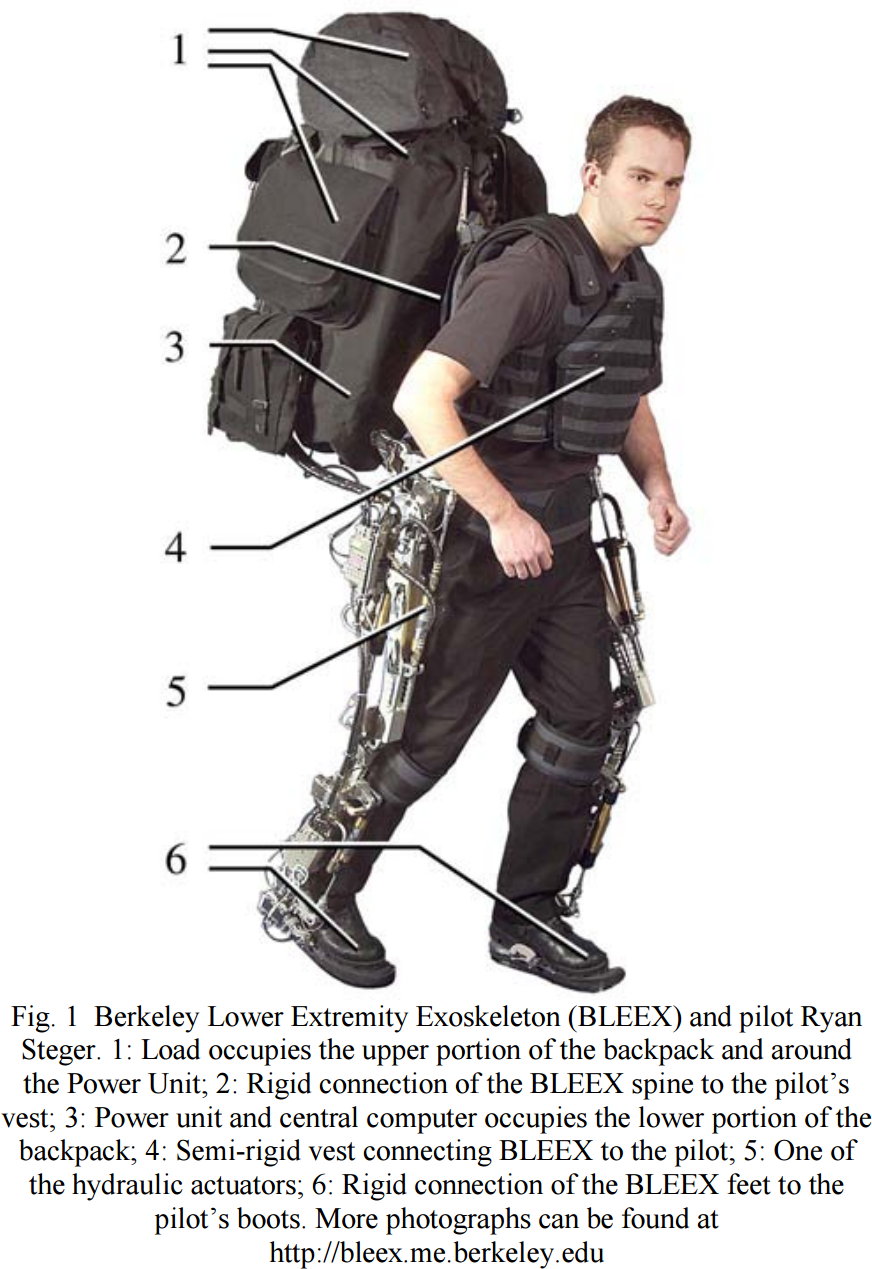
\includegraphics[width=3.5in]{exos/figs/bleex_exo.png}
\end{figure}

The BLEEX system includes two 7 DOF, three-segment legs with thigh, shank, and foot links, on-board power supply, and a backpack-like frame.  The human wearer is rigidly connected at the feet and torso such that the frame shelters the user by transferring load forces to the ground.  The leg segments are connected by rotational joints including 3 DOF (2 actuated) at the hip, 1 DOF (actuated) at each knee, and 3 DOF (1 actuated f/e in sagittal 
plane; 2 passive) at the ankles.  Joint angles, torque, and power requirements are determined from human motion analysis based on a 75-kg human walking on flat ground at roughly 1.3 m/s (the average military male's maximum reported joint limits are also used to derive joint range of motion targets).  During design, joint motion was intended to be slightly less than the maximum human range of motion for safety; however, some joint ranges had to be reduced to avoid singularities.
% Ideally, joint motion would provide the maximum human range of motion for safety

Due to its high power to weight ratio (twice that of electric motors), BLEEX uses a hydraulic actuation system.  An on-board internal combustion engine provides both electric and hydraulic power.  The joints are driven by commercial small bore (2cm) dual action hydraulic actuators operating at 6.9 MPa. Though the operating pressure is relatively low, the hydraulic actuation system exhibits significant pressures losses across servo valves when less pressure is required than this system pressure.  Table~\ref{tab:bleex_joints} provides details regarding the range of motion and torque capabilities of BLEEX's joints.  As reported in \cite{bleex_design_2006}, BLEEX requires 1,143 W for walking relative to 165 W for human walking (14\% efficient compared to a human of the same size).  Altogether the suit needs 2.27 kW of hydraulic power and 220 W of electric power to accommodate climbing (540 W) and remaining electrical loads including 240 W to power the second stages on servo vales.

%
\begin{table}
\centering
\begin{tabular}{|l|*{3}{c|}}  % repeats {c|} 6 times
\hline
& BLEEX & human max & BLEEX \\
& ROM & torque \& power & max torque \\ \hline
Ankle flexion / extension & $\pm 45^\circ$ & $-120$ N-m; 250 W & $-200 / 155$ N-m\\ \hline
Ankle abduction / adduction & $\pm 20^\circ$ & N/A & N/A \\ \hline
Knee flexion & $121^\circ$ & $-35 / 60$ N-m; $-150 / 50$ W & $-100 / 140$ N-m \\ \hline
Hip flexion / extension & $\pm 121^\circ / 10^\circ$ & $-80 / 60$ N-m; $-60 / 115$ W & $-150 / 130$ N-m \\ \hline
Hip abduction / adduction & $\pm 16^\circ$ & N/A & N/A\\ \hline
total rotation external & $35^\circ$ & N/A & N/A \\ \hline
total rotation internal & $35^\circ$ & N/A & N/A \\ \hline
\end{tabular}
\caption{BLEEX joint range of motion (ROM) is near anthropomorphic.  The max torques are designed to meet the torque / power requirements of similarly sized human walking at 1.3 m/s \cite{bleex_design_2006}.}\label{tab:bleex_joints}
\end{table}
%

\subsubsection{Control}

The BLEEX team has successfully implemented both sensitivity amplification \cite{sesitivityAmpPaper2005} and a hybrid assitive control scheme \cite{bleex_hybrid_control_2006} that switches (based on gait phase) between sensitivity amplification and a position control regulating desired torque. This section focuses on sensitivity amplification, as the hybrid assitive strategy did not perform as well in walking trials.

\begin{figure}[ht]
  \centering
  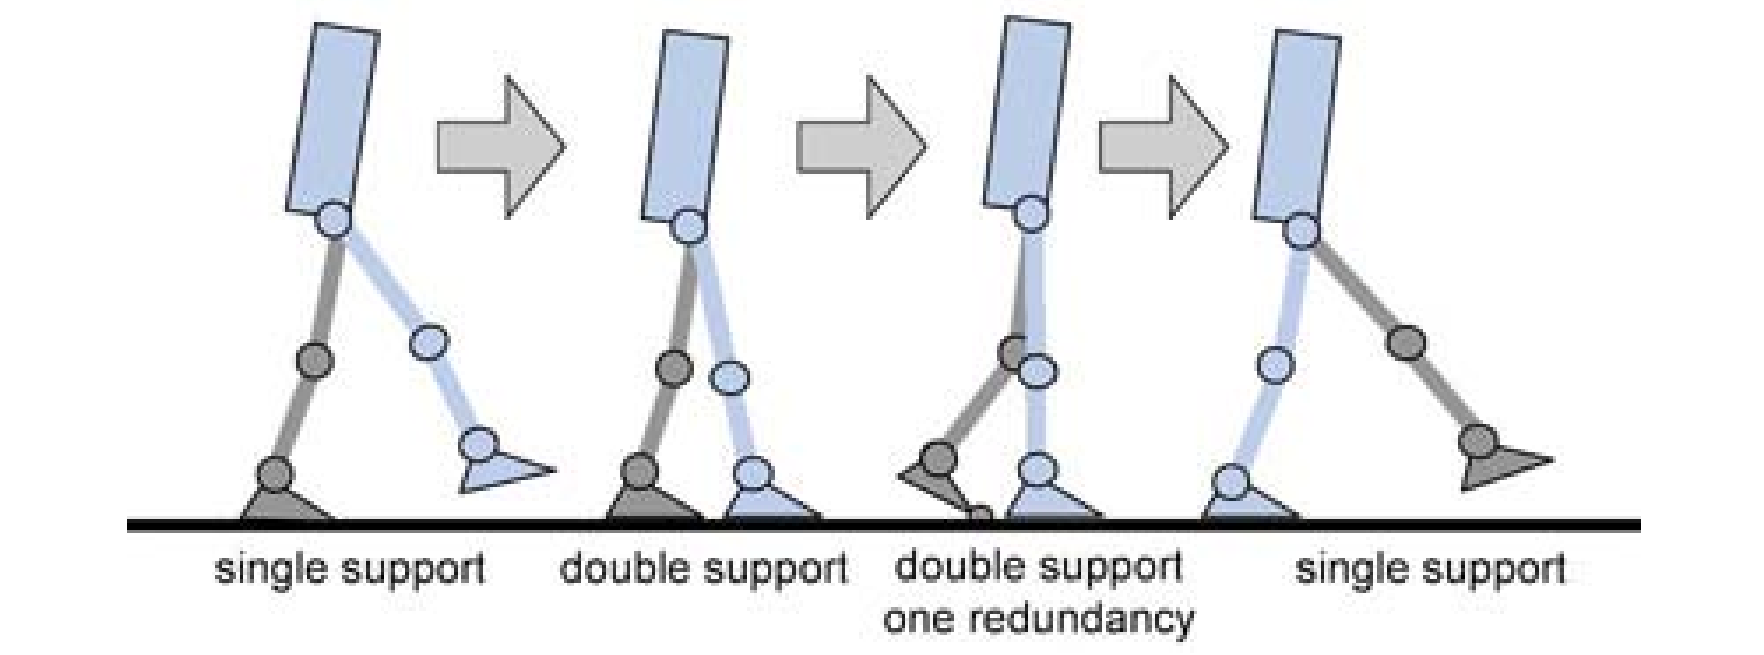
\includegraphics[width=3.5in]{exos/figs/bleex_support_phases.png}
\end{figure}

In its sensitivity amplification implementation, BLEEX controllers attempt to minimize interaction forces between the human pilot and the exoskeleton. However, the BLEEX team makes a point to avoid direct measurements of the interaction force between the human and the exoskeleton suit.  They highlight difficulties in properly outfitting humans with necessary sensing equipment and challenges in modeling the interaction between the human and exoskeleton (e.g., non-rigid, non-fixed contact points).  Instead, the team develops controllers based on an inverse dynamic model (in the saggital plane) of only the exoskeleton.  

\begin{figure}[ht]
  \centering
  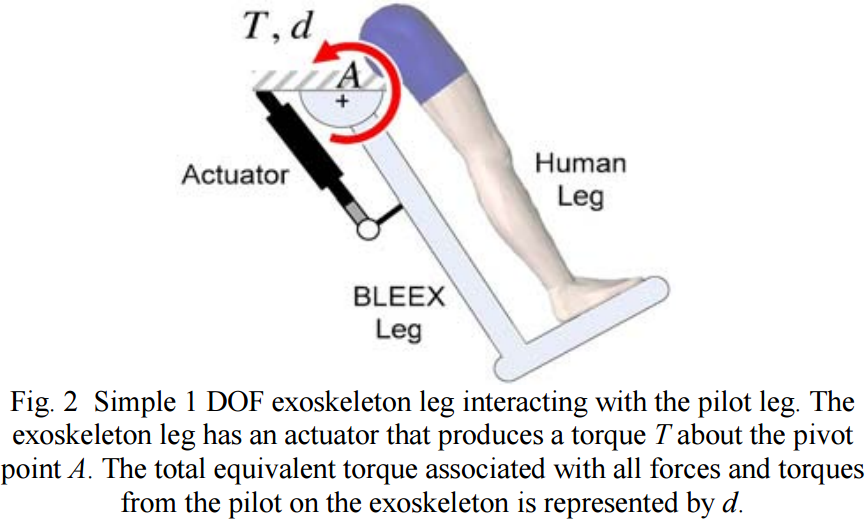
\includegraphics[width=3.5in]{exos/figs/bleex_1dof_ex.png}
\end{figure}

Assuming no outside disturbances, the BLEEX sensitivity amplification control strategy models the torque applied by the human pilot on the exoskeleton as $d$ (assuming no outside disturbances).   Neglecting gravity, the exokeleton angular velocity is modeled as 
\[v = G r + S d ,\] 
where $v$ represents the angular velocity of the exokeleton, $G$ is the transfer function from actuator inputs ($G$ is the exoskeleton's dynamics), $r$ is the actuator input, and $S$ is the sensitivity or transfer function from human torque to exokeleton angular velocity. 

\begin{figure}[ht]
  \centering
  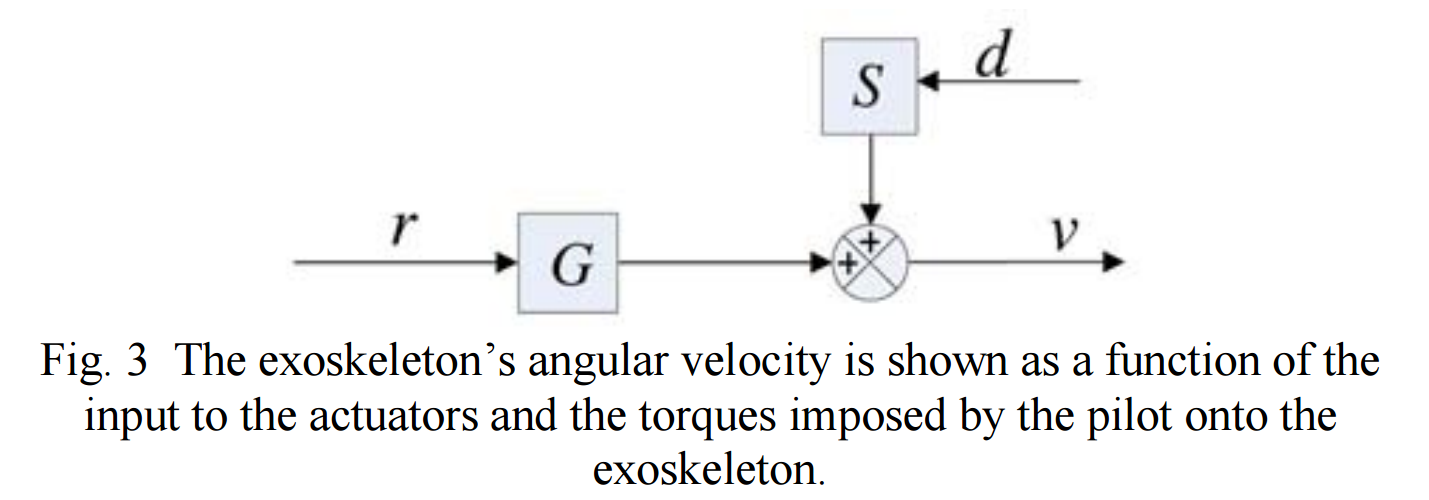
\includegraphics[width=4.0in]{exos/figs/bleex_control_diag_1.png}
\end{figure}

The goal is to maximize sensitivity to $d$ \emph{without direct measurement.}  Sensitivity amplification accomplishes this by creating a feedback loop from a controller, $C$, acting only on exoskeleton variables.  A new sensitivity equation,
\[S_{new} = \frac{v}{d} = \frac{S}{1 + G C} ,\]
is maximized by applying positive feedback.  To achieve a large sensitivity, BLEEX uses $C = (1-\alpha^{-1})G^{-1}$ so that $\alpha$ provides a direct (scalar) amplification factor. A low pass filter is often added to the $C$ term in order to damp out high frequency dynamics of the exoskeleton, which are not captured in these models.  Note that the controller depends on an inverse dynamic model of the exoskeleton, $G^{-1}$.  Since the model is hybrid, these dynamics switch according to gait phases (single support, double support, stance).  BLEEX detects these transitions using foot sensors.  Assuming the single leg support dynamics are in the form,
\begin{equation}
\mM({\bf\theta})\ddot{{\bf \theta}} + \mC({\bf\theta},\dot{{\bf\theta}}) \dot{{\bf \theta}} + \mV({\bf\theta}) = {\bf T} + {\bf d} ,
\end{equation}
where ${\bf T}$ is a vector of actuator torques, the BLEEX control torque would be
\begin{equation}
{\bf T} = \mV({\bf\theta}) + (1 - \alpha^{-1}) \big [ \mM({\bf\theta})\ddot{{\bf \theta}} + \mC({\bf\theta},\dot{{\bf\theta}}) \dot{{\bf \theta}} \big ] .
\end{equation}
The user must provide the first torque component as the exoskeleton has no actuator acting between the foot and the ground (the system is underactuated).

\begin{figure}[ht]
  \centering
  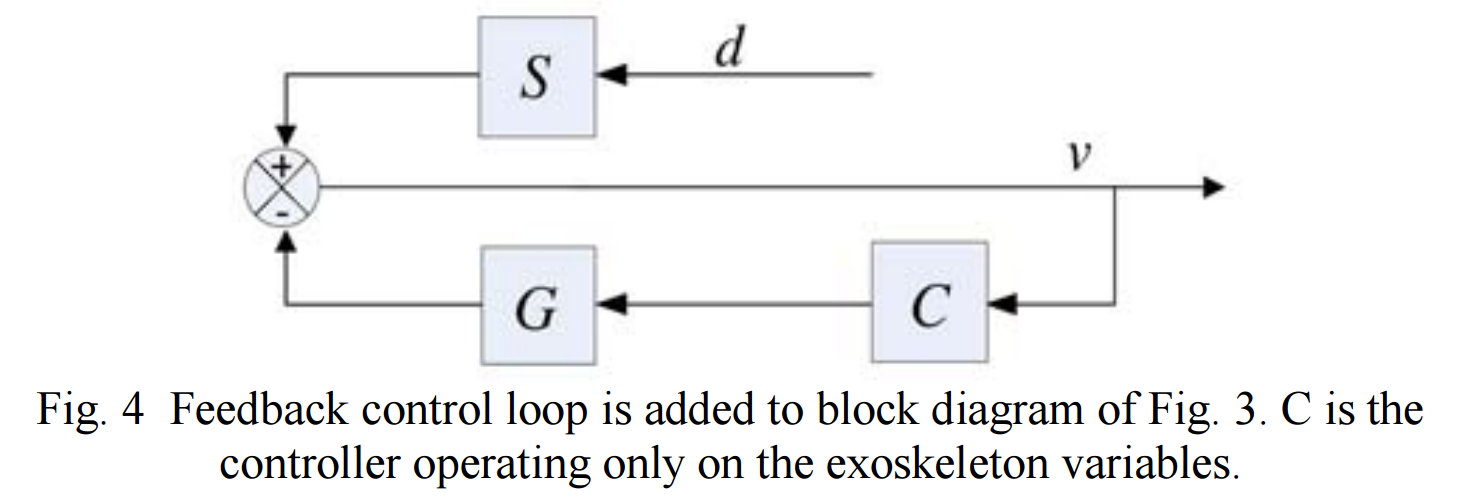
\includegraphics[width=4.0in]{exos/figs/bleex_control_diag_2.png}
\end{figure}

As a note, positive feedback is normally avoided in control design because it amplifies disturbances.  In the case of BLEEX, designers sacrifice disturbance rejection to maximize the response of the suit to its wearer.  Users must therefore take action to stabilize and balance out disturbances.

\begin{figure}[ht]
  \centering
  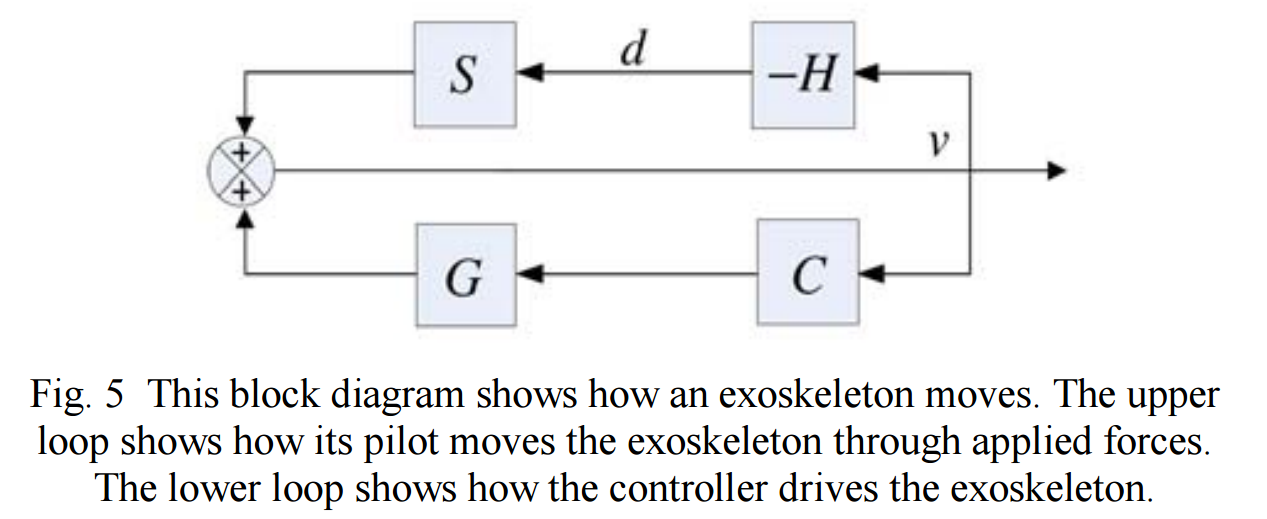
\includegraphics[width=4.0in]{exos/figs/bleex_control_diag_3.png}
\end{figure}

For sensing, BLEEX uses information from \textbf{8 encoders} and \textbf{16 accelerometers} to determine angle, angular velocity, and angular acceleration of eight actuated joints. It includes a \textbf{foot switch and load distribution sensor} at each foot. Eight single axis \textbf{force sensors} provide measurements required to perform low level force control at each actuator. An \textbf{inclinometer} indicates the orientation of the backpack relative to gravity. Using this sensitivity amplification control scheme, BLEEX has achieved successful walking at 1.3 m/s with a 34kg payload \cite{sesitivityAmpPaper2005}.

\subsection{Assessment and Recommendations}

Sensitivity amplification is a current best-in-class control strategy.  The exoskeleton shadows the user and uses exoskeleton data for joint angle, velocity, and acceleration and the exoskeleton model to minimize torques experienced by the human torque.  The process and hardware are relatively simple yet effective.   However, the approach has several significant disadvantages including heavy reliance on an accurate exoskeleton model and the fact that sensitivity amplification will amplify disturbances.  Note that in combat situations this latter point is critical as a sensitivity amplification will amplify forces acting on the suit and the operator will have to re-act to compensate.  The only way to compensate for or resist external forces in this setting is to filter them out, which would be extremely challenging unless additional sensory equipment is provided.  As one possibility, a sensitivity optimization approach may be paired with sEMG data to estimate user intent and provide such a filter.  Note this type of implementation would present its own challenges considering limitations in sensing and calibration of current EMG systems. 


\bibliographystyle{plain}
\bibliography{exos/bleex}

The figures in this section were obtained from \cite{sesitivityAmpPaper2005}. Materials presented are based on the references above.


\section{HAL}
\label{exo:hal}
\begin{refsection}[exos/hal.bib]

% keywords: model-based control; predefined gait trajectory; strength augmentation; rehabilitation.\\

The hybrid assistive limb (HAL) exoskeleton is developed by the University of Tsukuba and Cyberdyne for human strength augmentation and as an assistive gait device in rehabilitation.  Although several prototypes have been developed, this section focuses on the most recent HAL-5 model (specifically the non-clinical type, HAL-5 Type-B). Though HAL-5 is a full body exoskeleton, only hip, knee joints, and ankle are actuated in the sagittal plane.  The exoskeleton uses DC motors with harmonic drives at hip, knee, ankle joints (in some models the ankle joints act as passive springs).  HAL weighs 23kg and includes an on-board AC100V battery as the power source, which is designed to support maximum velocity human walking and standing torque requirements.  The battery allows for 160 min of continuous operation and enables the exoskeleton to lift up to 70kg \cite{HALassist2011}.  

Human operators attach to HAL at the waist with a belt, and at the calf and thigh using harnesses. HAL's frame does not transfer load to the ground.  Instead, HAL adjusts hip, knee and ankle torques to amplify its operator's torque. The exoskelton's sensory system includes bioelectric sensing (including \textbf{sEMG}), \textbf{angular sensors}, \textbf{acceleration sensors}, and \textbf{center of pressure / center of gravity} (COP/COG) sensors.  COP/COG sensing is provided through shoes with ground reaction force sensors.  The joint measurements are provided by potentiometers.
In at least one version of HAL the bioelectric data comes from sEMG sensors installed below the operator's hip and above the knee (on both front and back).
An IMU installed in HAL's backpack is used to estimate torso pose.


\begin{figure}[ht]
  \centering
  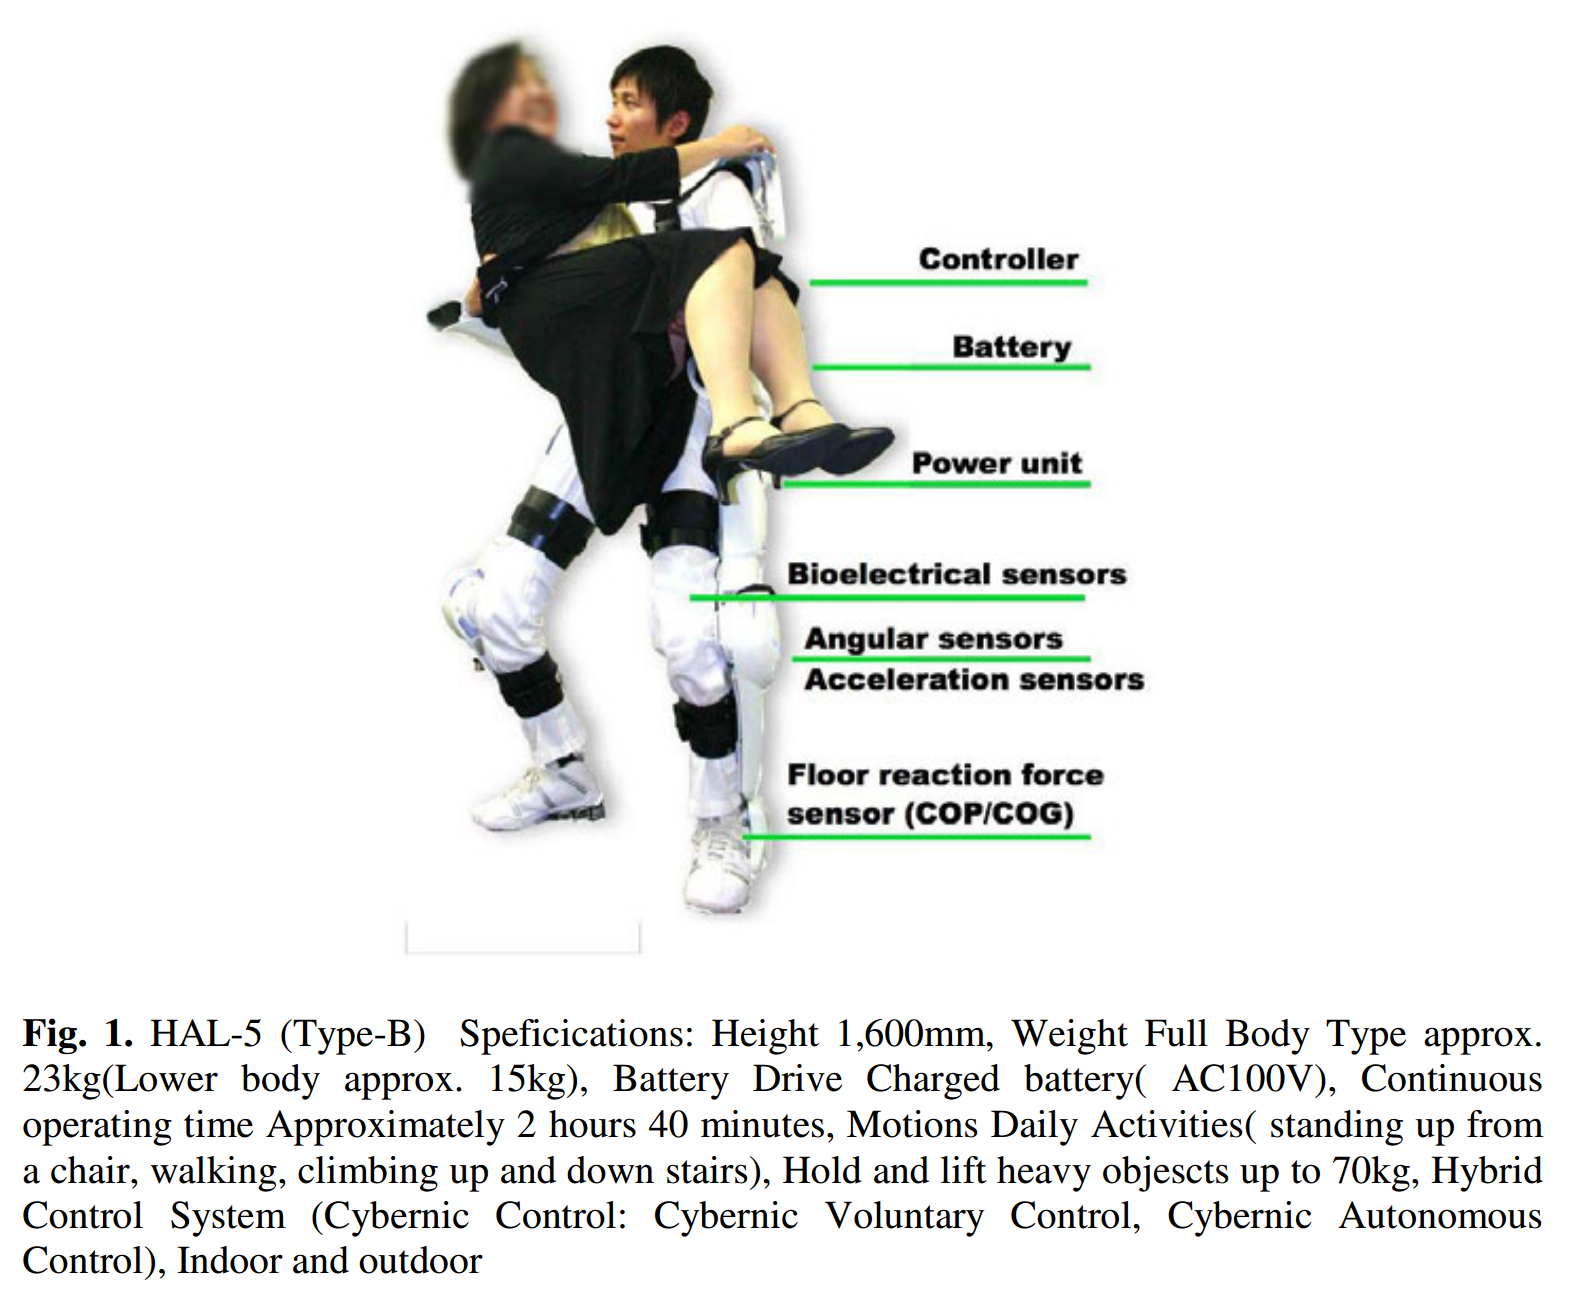
\includegraphics[width=3.5in]{exos/figs/hal-5_B_diagram.png}
\end{figure}


\subsubsection{Control}

HAL has two types of control systems designed for different application domains.  For gait assistance and rehabilitation, HAL uses an autonomous control system that carries the user through predefined gait trajectories by controlling knee and hip joints (the ankles behave as passive springs).  Gait phase intention is estimated from COP/COG sensors.  The exoskeleton drives the wearer to follow pre-recorded desired joint patterns.

The second control strategy, a model-based approach for human strength augmentation, estimates human intention from sEMG activity and provides power to augment torque provided by the operator.  A relatively autonomous torque assist strategy in \cite{HALmodelControlKnee2010} recognizes user intention to take a step by thresholding sEMG data.  The approach provides a knee torque response including an assitive torque component, a viscous damping component that reduces high velocity motion for safety, and a gravity compensation torque.  
%In \cite{HALvTorqueImp2002}, HAL uses myoelectric data to estimate muscle torque based on the difference between flexor and extensor muscle activities.  

In \cite{HALmuscleImped2005}, an impedance control strategy controls the viscoelastic properties of HAL's knee joint from a musculoskeletal model of operator's limb moving in concert with the exoskeleton.  The controller uses sEMG sensor data to estimate muscle torque based on the difference between flexor and extensor muscle activities.  The authors note the sEMG model requires significant calibration effort.  
Viscoelastic torques are computed according to
\[\tau_{a,i} = \alpha_i(-D_i \theta_i - K_i \theta_i),\]  
based on a variable gain set by $\alpha_i$.  The net knee actuator torque is
\[\tau_i = \tau_{a,i} + \tau_\mu + \tau_c .\]
The torque includes a $\tau_c$ term compensating for mechanical (actuator) impedance and $\tau_\mu$, a scaled version of the human torque (as estimated  from sEMG data).  The $K_i$ and $D_i$ terms in $\tau_{a,i}$ are viscoelastic parameters (based on the operator's muscles) in the human-exoskeleton model.  These parameters are estimated on-line using a weighted least-squares method.  In this case, the angular velocity data required for the impedance controller is estimated from a state observer.

%
\begin{figure}[ht]
  \centering
  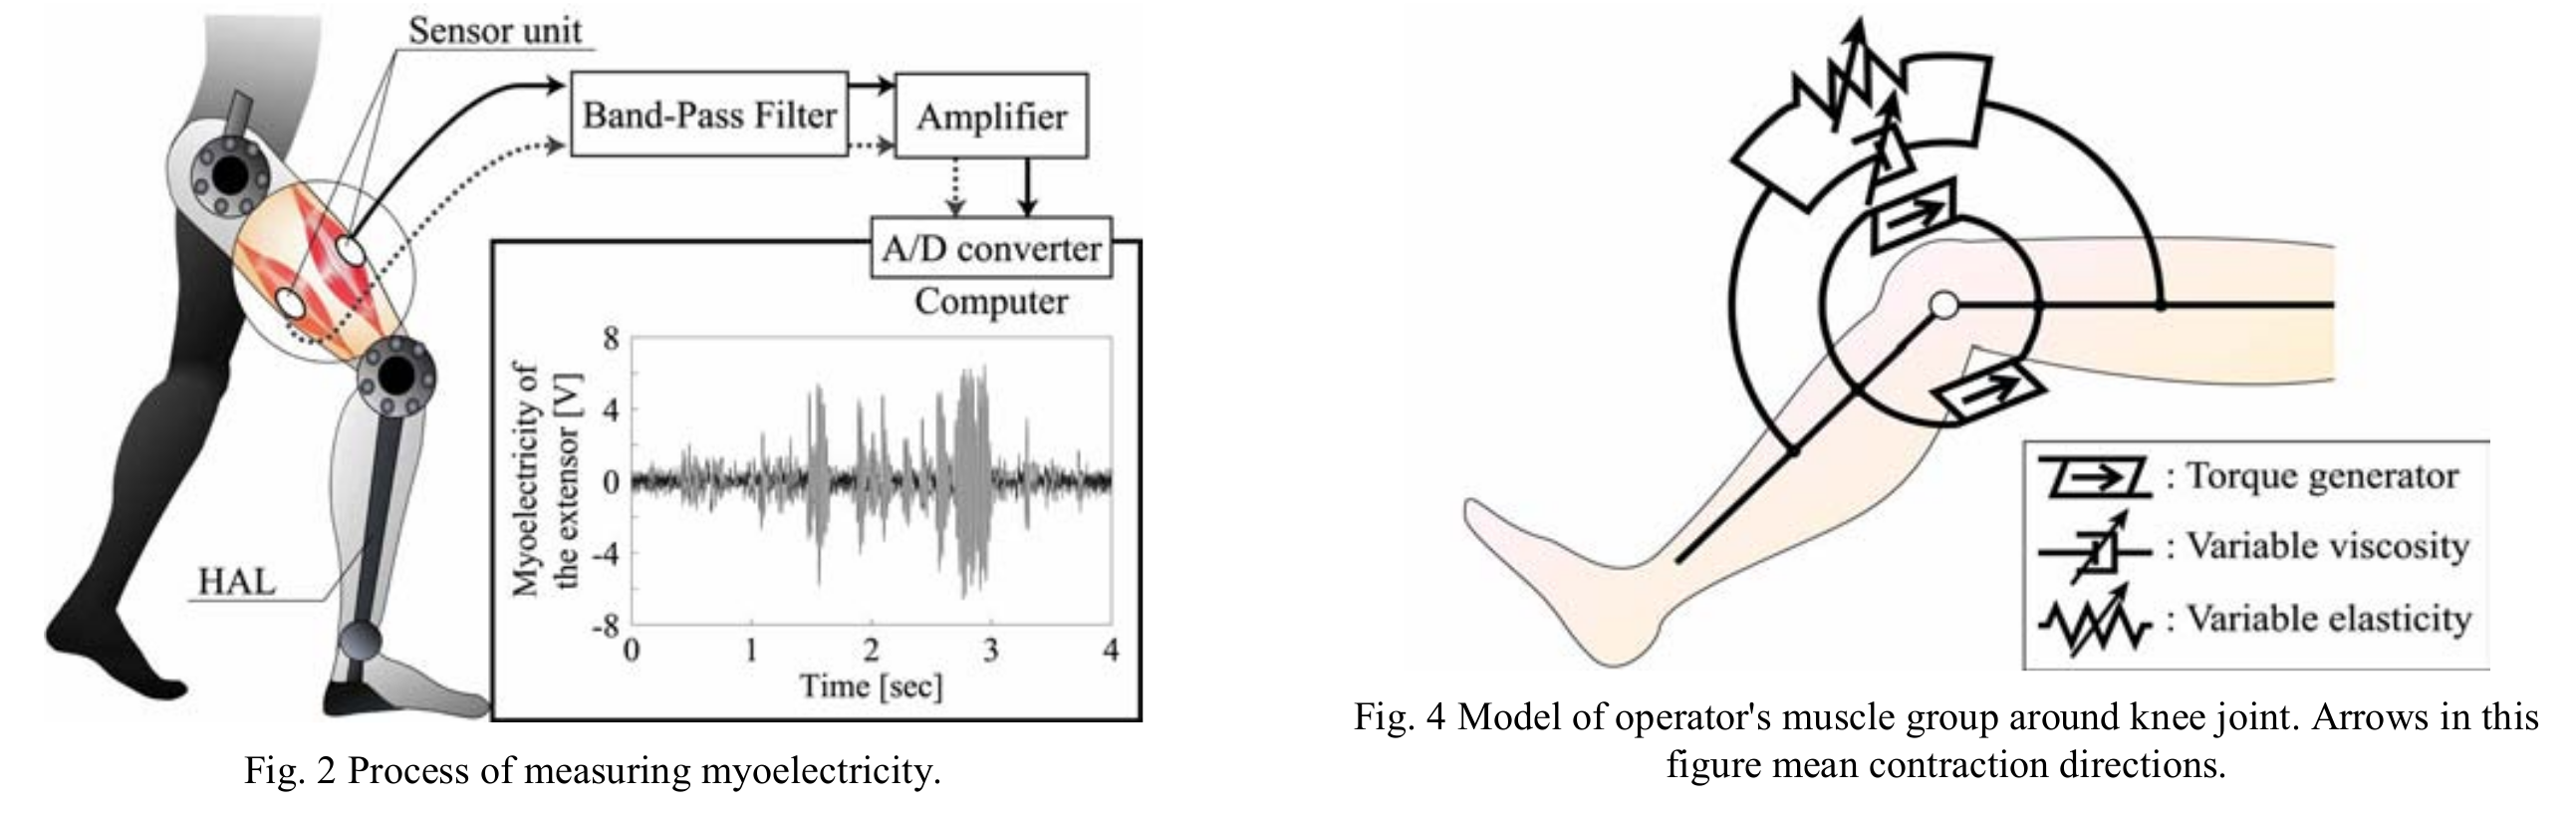
\includegraphics[width=6in]{exos/figs/hal_viscoelastic_control.png}
\end{figure}
%
%

While experiments in \cite{HALmuscleImped2005} only consider leg swing-up and swing-down, a similar control approach in \cite{HALvTorqueImp2002} switches the dynamics based controller to compensate for swing and stance phases in walking gait.  In this case, the gait transitions are detected by thresholding foot sensors and required angular velocity (and acceleration) data are determined by numerically differentiating angular encoders.


\subsection{Assessment and Recommendations}

Compared to sensitivity amplification methods, HAL's use of EMG data allows it to estimate intention without amplifying external disturbances.  While direct sensing of user intention is ideal for noisy, contract-rich environments, sEMG data is extremely difficult to work with due to high filtering and calibration requirements.  A hybrid strategy which uses sensitivity amplification and sEMG data (possibly thresholded) to filter user intention could prove effective.  Additionally, Section~\ref{survey:recommend} mentions new capabilities in nano-fabrication and MEMs technologies that have produced new high-density, wearable sensing arrays. These and similarly advanced sensing technology may facilitate direct measurement of interaction forces (i.e. estimating pressure / force and exoskeleton contact locations), which could potentially filter external disturbances from user generated input to estimate intent.

\nocite{*}
\printbibliography[heading=subbibliography]

The figures in this section were obtained from \cite{HALmuscleImped2005,HALassist2011}.  Materials presented are based on the references above.

\end{refsection}




%%% Local Variables:
%%% mode: latex
%%% TeX-master: "../survey"
%%% End:


\section{XoR}
\label{exo:XoR}
\begin{refsection}[exos/xor.bib]

keywords: model-based control; strength augmentation; hybrid actuation; pneumatic actuation; electric motors;\\

\begin{figure}[ht]
  \centering
  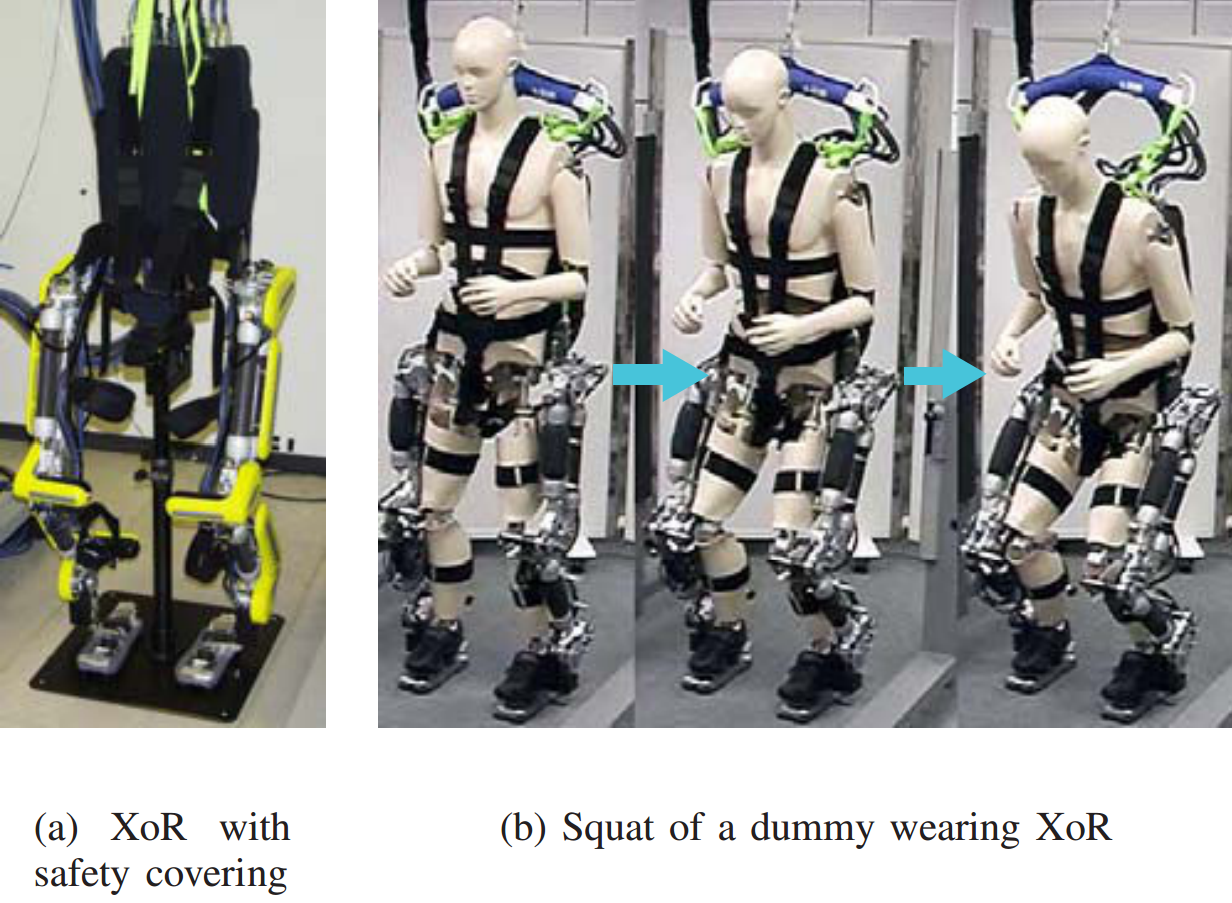
\includegraphics[width=4.0in]{exos/figs/xor.png}
\end{figure}

The XoR is a prototype, light-weight lower-body exoskeleton that uses a hybrid pneumatic-electric drive system that \textbf{reduces weight} while providing \textbf{precise torque control}, \textbf{backdrivability}, and a \textbf{desirable force / velocity} profile.  The exoskeleton is designed to serve in rehabilitation settings to augment operators' strength and assist with postural control for persons with disabilities.

\begin{figure}[ht]
  \centering
  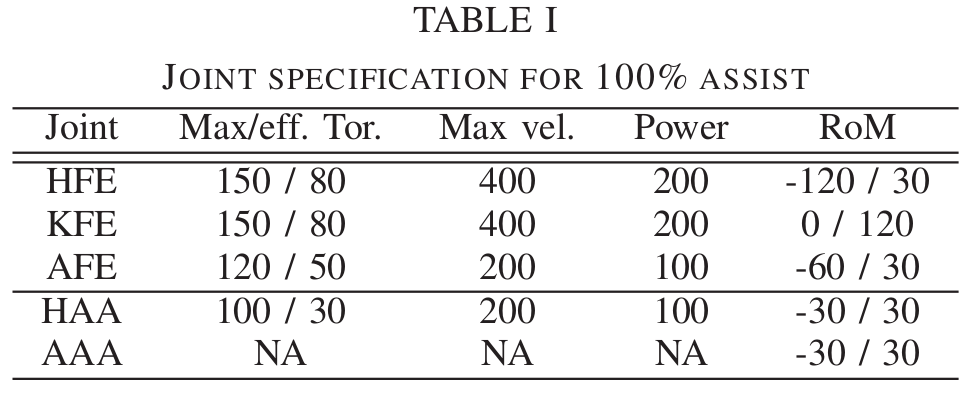
\includegraphics[width=3.5in]{exos/figs/xor_joint_rom.png}
\end{figure}

The XoR weighs 30kg and includes 10 DOF with 6 active joints (flexion / extension of hip, knee, and ankles) and 6 passive (hip abduction/adduction joints, hip rotation, and ankle adduction/abduction).  The active joints are powered by hybrid actuators comprised of an \emph{air muscle} and an electric motor.  The hybrid actuation scheme uses a unilateral air muscle layout to compensate for gravity and bilateral electric motors with relatively small gear ratio (57.5) to serve as the dynamic compensator.

The actuation scheme is complementary in that the electric motors have a quick response time and produce high peak torque for short amounts of time, while air muscles have a delayed response (true of pneumatic systems in general due to the compressibility of air) with better power density and sustained torque.  The hybrid drive system sums the two to develop a desired torque profile that achieves the benefits of both and reduces weight and motor size.  The system offers high torque control with negligable stick-slip and backdrivability.

\begin{figure}[ht]
  \centering
  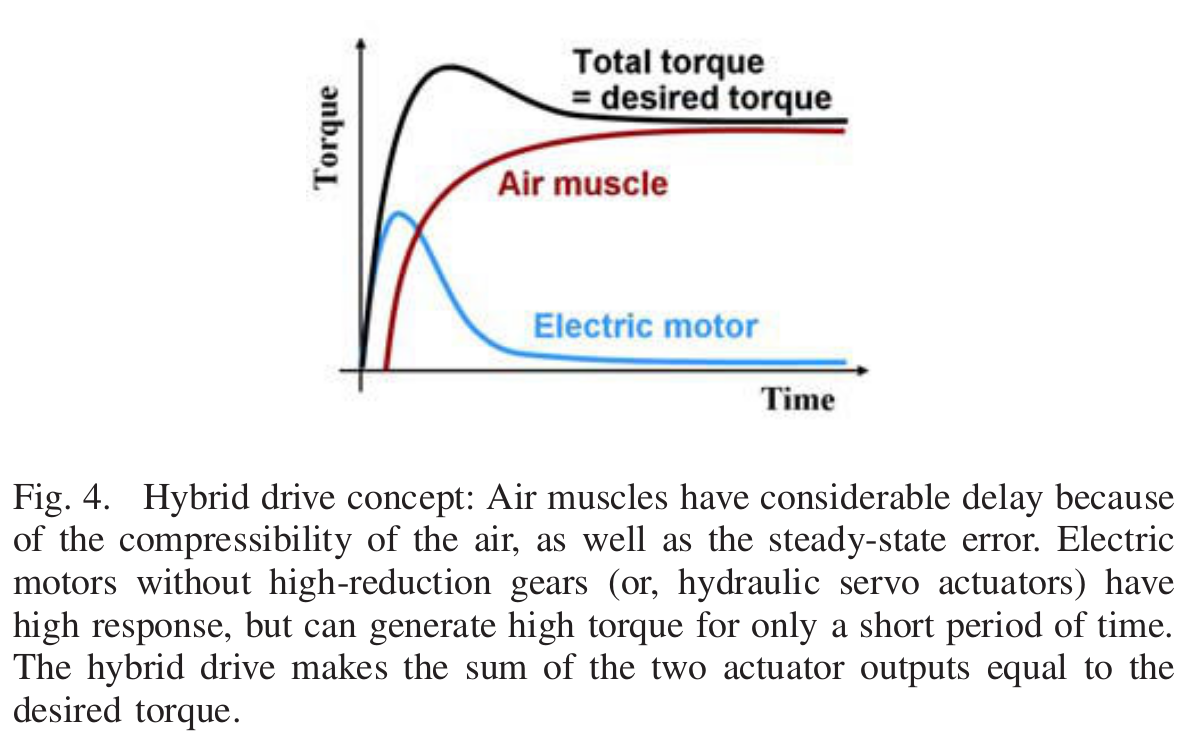
\includegraphics[width=3.5in]{exos/figs/xor_hybrid_drive_torque_time.png}
\end{figure}  

A challenge in using air muscles is that force reduces quadratically as a function of contraction.  For instance, at 30\% contraction, the force produced by FESTO rubber air muscles vanishes.  To address the issue, XoR is strategically places air muscles to generate forces in desired configurations.  

\begin{figure}[ht]
  \centering
  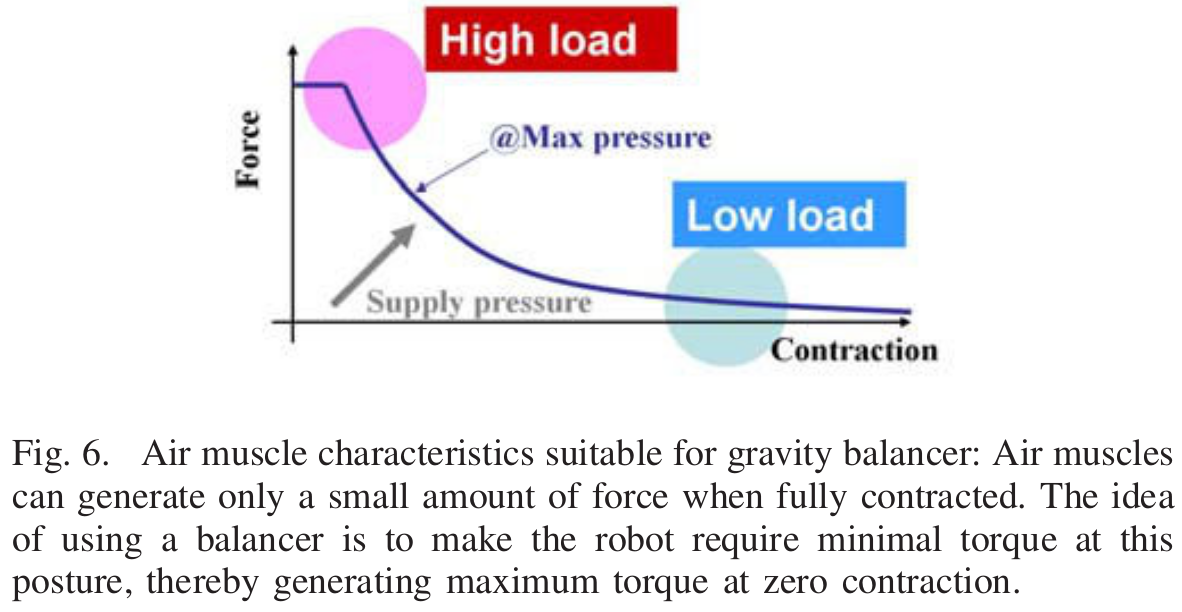
\includegraphics[width=3.5in]{exos/figs/xor_air_muscle_force_vs_contraction.png}
\end{figure}

In implementation, the XoR uses rubber air muscles (MDSP-40) connected to pulleys via tendons and to EP regulators in the backpack (a constant pressure and cam system is being tested to reduce weight required for backpack air valves).  The electric actuator is a geared, 200W brushless DC motor (Maxon EC powermax 30) rated at 4.7 A, which transmits power to joints through a belt and pulley system with a 57.5 gear ratio. the motor's 0.12 Nm output torque provides up to 34.5 Nm (for short duration) at every joint and is backdrivable.  The design yields a relatively high range of motion (up to 120 degrees) with a load capacity 150 Nm.  However, experiments reveal the need for bi-directional pneumatic actuation at hip joints.

For sensing, XoR is equipped with rotary encoders at joints, an IMU in the backpack, load cells in the feet, and is networked to servers capable of providing EMG, NIRS, and EEG data.  A control PC running at 1 KHz, pulse counter, amplifiers, Digital IO are external and so not included in the weight of the unit.  Human operators are outfitted with a goniometer.


\subsubsection{Control}

The XoR control strategy applied in \cite{XoRkinemExtraction2012} has two main components.  First, a proportional-derivative (PD) feedback controller tracks desired joint angles and angular velocities that correspond to the state of the exoskeleton required to assist the human operator.  To obtain this state (specifying the desired joint angles / velocities), the controller simultaneously measures the joint angle trajectories of the human user (goniometer) and of the robot (encoders), and uses canonical correlation analysis (CCA) to extract latent variables in the kinematic relationship between the two.

\begin{figure}[ht]
  \centering
  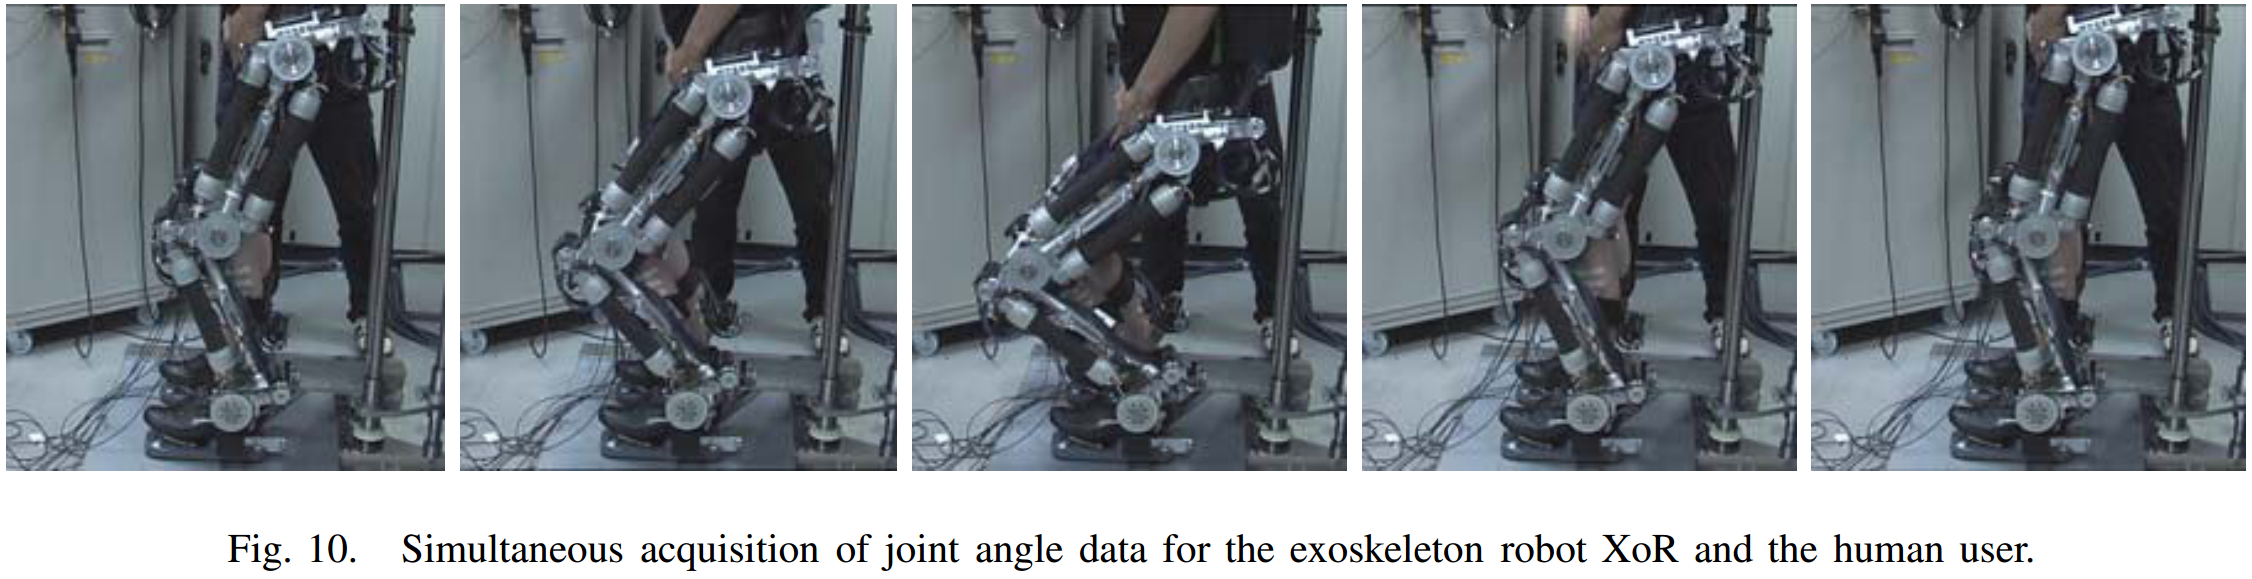
\includegraphics[width=6.0in]{exos/figs/xor_joint_angles.png}
\end{figure}

To avoid relying on high gain feedback, XoR incorporates user intent through EMG data.  The controller rectifies and low pass filters (10 Hz cut-off) data measured in the pilot's quadriceps femoris, tensor fasciae latate, gluteus medius, and tibialis anterior. 
It sets desired joint angles and velocities, ${\bf x} = ({\bf \theta} \dot{\bf \theta})$, from the EMG data, ${\bf u} = (EMG_1 \cdot EMG_n)$, using a linear prediction model, 
\[{\bf x}(k+1) = \mA{\bf x}(k)+\mB{\bf u}(k),\].  
The controller uses the angular measurements required to perform CCA and EMG data to derive the model's $\mA$ and $\mB$ terms.  The predicted state from EMG model provides the desired input to yet another PD controller: 
\[\tau_i = K_p (\theta_i^d - \theta_i) + K_d (\dot\theta_i^d - \dot \theta_i),\] 
with gains of $K_p = 1000$ and $K_d = 100$.

In hip tracking experiments, the team found EMG data to be helpful.  When using EMG signals, XoR achieved a mean squared error of $1.8E^{-3}$.  Without the EMG data, the mean squared error increased to $2.1$.  Additional experiments confirm the air muscles can effectively perform gravity compensation when used in conjunction with electric actuators (to correct for torque errors induced by inaccuracies in the model mapping position to toque in air muscles).


\subsection{Assessment and Recommendations}

The XoR prototype uses a promising hybrid actuation scheme to achieve both fast peak torque response and higher sustained torque while remaining lightweight.  They track human motion with feedback from a goniometer and feedforward control provided by EMG data.  These human intention / sensing modalities are both difficult to implement due to noise and calibration issues.  However, capturing the user intent is important, especially in the presence of external disturbances.  If the sensory system were improved (e.g, wearable ``robot skin'' sensing arrays), this exoskeleton design could be highly effective. 

\nocite{*}
\printbibliography[heading=subbibliography]

The figures in this section were obtained from \cite{xorDesign2011,XoRkinemExtraction2012}. Materials presented are based on the references above.

\end{refsection}

\subsection{EXO-UL7}
\label{exo:exo-ul7}

keywords: model-based control; strength augmentation;\\

\begin{figure}[ht]
  \centering
  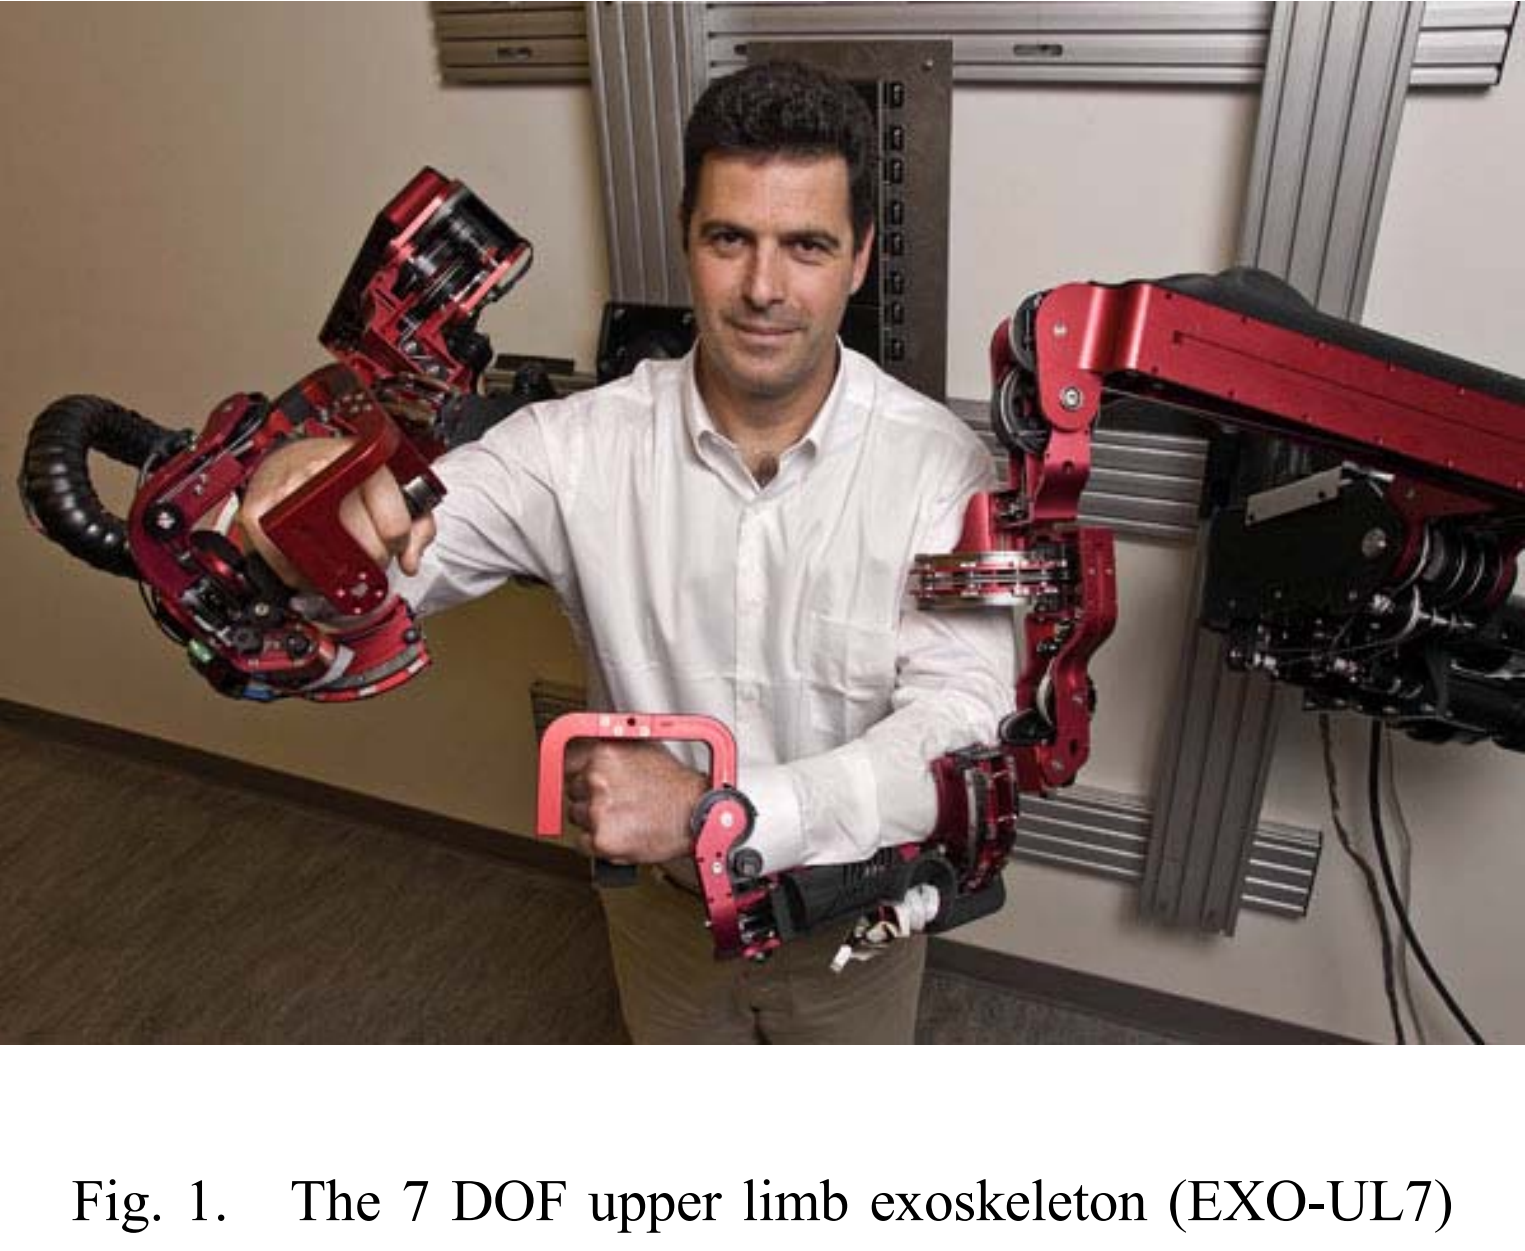
\includegraphics[width=4.0in]{exos/figs/exo-ul7.png}
\end{figure}


Although this study focuses on lower-body exoskeltons, we include the EXO-UL7 7 DOF upper-extremity exoskeleton for its novel actuation scheme and principled design. 

-------------------------------------------------

(Called CADEN - "cable driven dexterous exoskeleton for neurorehabilitation" in [[EXOul7design]])

Design:

7 DOF model; cable-actuated; proximal motor placement and distal cable-pulley reductions for low inertia, high stiffness links with backdrivable transmissions with zero backlash.  "Enables full glenohumeral, elbow, and wrist joint functionality." -- [[EXOul7design]]

% set the Human Machine Interface (HMI) at the neuromuscular level ... as one of the primary command signals... Use sEMG signals.  -- http://bionics.seas.ucla.edu/research/exoskeleton_device_3.html

[[EXOul7design]] contains data from a dynamic / kinematic study of human motion during everyday tasks in order to determine design requirements for exo.

3 lvls of safety mechanisms: 1) built in mechanical -- phys. stops, 2) electrical -- three wearer e-stops including an observer e-stop, an enable button which must be held, and a foot switch e-stop, and 3) software -- redundant position sensing (pots, Midori, Fullerton; shaft encoder, HP), one at either side of power train, monitor both joint motion and motor position. -- [[EXOul7design]]

Control bandwidth -- targeted 10Hz based on achievable frequency range of human arm which is btwn 2Hz and 5Hz.  They found shoulder joint had 1st resonant mode at 6 Hz. -- [[EXOul7design]]

Weight: 3.5 and 6kg from links 1 and links 2-7 (resp.). -- [[EXOul7design]]

Articulation: 7 single axis revolute joints.  Use three pulleys (90 and 180 deg configurations) at joints to keep cable length constant. Stack of pulleys required -- two pulleys representing agonist muscle groups and two for antagonist -- [[EXOul7design]]

Singularities: Design movable joint mechanisms that allow adjustment of singularity within 15deg based on user preferences. -- [[EXOul7design]]

Power transmission: shafts, cables, fluid lines, and gear trains.  Use pulleys for speed reductions and backdrivability.  2-stage pulleys in proximal joints 1-4 and single stage for more distal (5-7). -- [[EXOul7design]]

Motors for joints 1–4 were mounted on the stationary base, achieving a 60% reduction in overall weight of the moving parts. The remaining three motors, whose torque requirements are substantially less, were positioned on the forearm -- [[EXOul7design]]


Control Strategy:

Model-based control -- "proposed HMI takes advantage of the electro-chemical-mechanical delay, which inherently exists in the musculoskeletal system, between the time when the neural system activates the muscular system and the time when the muscles generate moments around the joints. The myoprocessor is a model of the human muscle running in real-time and in parallel to the physiological muscle.   During the electro-chemical-mechanical time delay, the system will gather information regarding the physiological muscle’s neural activation level based on processed sEMG signals, the joint position, and angular velocity, and will predict using the myoprocessor the force that will be generated by the muscle before physiological contraction occurs. By the time the human muscles contract, the exoskeleton will move with the human in a synergistic fashion, allowing natural control of the exoskeleton as an extension of the operator's body." %-- http://bionics.seas.ucla.edu/research/exoskeleton_device_3.html

Say they use neuro control strategy to avoid having to trigger motion based on human movement / force (required in position, force-impedance control) -- [[EXOul7design]]


References:

Cavallaro E., J. Rosen, J. C. Perry, S. Burns, B. Hannaford, Hill Based Model as a Myoprocessor for a Neural Controlled Powered Exoskeleton Arm – Parameter Optimization, Proceedings of the 2005 IEEE international Conference on Robotics and Automation, ICRA 2005, pp. 4525 – 4530, Barcelona Spain, April 2005

Rosen J,, J. C. Perry, N. Manning, S. Burns, B. Hannaford, The Human Arm Kinematics and Dynamics During Daily Activities – Toward a 7 DOF Upper Limb Powered Exoskeleton, - ICAR 2005 – Seattle WA, July 2005. [ CP19]

Perry J.C., J. Rosen, Design of a 7 Degree-of-Freedom Upper-Limb Powered Exoskeleton Proceedings of the 2006 BioRob Conference, Pisa, Italy, February, 2006.

Cavallaro E., J. Rosen, J. C. Perry, S. Burns, Myoprocessor for Neural Controlled Powered Exoskeleton Arm, IEEE Transactions on Biomedical Engineering, pp. 2387-2396, Vol. 53, No. 11, November 2006

Perry J. C., J. Rosen, S. Burns, Upper-Limb Powered Exoskeleton Design, IEEE Transactions on Mechatronics, Volume 12, No. 4, pp. 408-417, August 2007 <<EXOul7design>>

Rosen J., and J.C. Perry, Upper Limb Powered Exoskeleton, Journal of Humanoid Robotics, Vol. 4, No. 3 (2007) 1–20

Miller, L.M. and J. Rosen, 2010." Comparison of multi-sensor admittance control in joint space and task space for a seven degree of freedom upper
limb exoskeleton," 3rd IEEE RAS and EMBS International Conference on Biomedical Robotics and Biomechatronics (BioRob). <<EXOul7admitJointTaskCmp>>

Wen, Y., J. Rosen, and L. Xiaoou, 2011." PID admittance control for an upper limb exoskeleton," American Control Conference (ACC).  <<EXOul7admit>>

-------------------------------------------------

\subsection{Assessment and Recommendations}

The EXO-UL7 is a well-designed upper body exosekelton that is experimenting with new sEMG based control mechanisms.  The control approach is not as refined and needs to be developed further before field applications due to reliance on sEMG data.  
% As mentioned in Sections~\ref{exo:bleex} and \ref{exo:hal}, there are advantages to .


The figures in this section were obtained from \cite{EXOul7design2007,EXOul7pidAdmit2011}.  Materials presented are based on the references above.


\section{Discussion}

Discussion to be written.

\section{Conclusions and Recommendations}

Conclusions and Recommendations to be written.

1) We recommend a particular control 
overall architecture in Section~\ref{sec:architecture}.
We do not expect this to be controversial.

2) We recommend actuation that can be treated as force or torque sources.
This is a potentual problem for revolute electric actuation, as it
is difficult to get necessary performance at low gear ratios (20-50)
and fit the necessary torque sensing,

3) We recommend the use of dynamic models of the exoskeleton, as has been done
for the last decade starting with the BLEEX exoskeleton.
We do not expect this to be controversial.

4) We recommend using online optimization as part of the Lowest Level Controller
in the form of quadratic programming. Online optimization
was tested by the top biped robot
teams in the DARPA Robotics Challenge, and worked well.
A possible objection to online optimization
is that it requires more substantial computing
resources than current exoskeleton control methods. We feel the feasibility
of this approach has been demonstrated and is easily achievable. Perceptual
computing costs will dwarf computing costs for control, 
so the computation cost is a non-issue.

5) We recommend applying as many sensors as possible, and asking the performers
to make it easy to add more by making the sensor network available in the design.
This maximizes the probability of success
with respect to control architectures and algorithms by enabling multiple control
approaches to be implemented, refined, and support each other.
In particular, we would like to see force sensing between the operator and the
exoskeleton, including at the feet, as much force sensing between the exoskeleton 
and the world as possible, but minimally full six-axis force/torque sensing at
the exoskeleton feet (where they touch the ground). We would like to see multiple MEMs
IMUs (measuring linear acceleration and angular velocity) installed across 
the exoskeleton and at least one high quality fiber optic gyro IMU. 
We would like to see high quality direct velocity sensing
such as high count (100,000 counts/revolution) encoders and/or 
analog rotary or linear tachometers on actuators and joints. 
We would like to see actuator force or torque sensors
(load cells or equivalents) with the measurement on the link side (rather than
the actuator side) of any transmission. Electric current in motors and oil
pressure in hydraulic pistons can also be used for actuator force estimation,
but because these measurements are on the actuator side before the transmission
and in the case of hydraulics before the oil seals on the piston, these measurements
are greatly contaminated by friction. On the Atlas humanoid we typically saw 10Nm
joint torque estimation errors for a system that estimated actuator output using
oil pressure on each side of the piston head.
A possible objection to this is additional cost. We feel it is a false
economy to skimp on sensing. Leaving practical sensing out greatly increases
the risk of poor performance.

6) We recommend a ``symbiotic'' control system design should be used as a backup,
in case more aggressive design philosophies such as ``invisible'' and ``natural''
control system designs are not achievable.,
The ``symbiotic'' control system design
expects the operator to adapt to the exoskeleton and its control,
and has the control customized for the operator.

7) We recommend making use of virtual model control specialize
for the various tasks. This can greatly increase operator/exoskeleton system
performance over an exoskeleton that just carries a load and is otherwise
``invisible''.

\bibliographystyle{plain}
\bibliography{exo}

\end{document}




sensitivity to
 modeling error
 sensor error
 unmodeled dynamics

underactuated control problem
 - not fully actuated sagittal only.
 - how necessary is lateral actuation
 - what is the penalty
  weight
  drag of actuator

how handle failure and damage after Oct 1

what about a full model of the system

Oct 5-9

%%% Local Variables:
%%% mode: latex
%%% TeX-master: t
%%% End:
